\documentclass{article}
\usepackage[utf8]{inputenc}
\usepackage{titlesec}
\usepackage{tikz}
\usepackage{amsmath}
\usepackage{booktabs}
\usepackage{graphicx}
\graphicspath{ {images/} }
\usepackage{tikz,pgfplots}
\usepackage{indentfirst}
\usepackage{braket}
\usepackage{float}
\usepackage{times}
\usepackage{hyperref}
\usepackage[english]{babel}
\usepackage{graphicx}
\usepackage{gensymb}
\usepackage{siunitx}
\usepackage{float}
\usepackage{amsmath}
\usepackage{caption}
\usepackage{subfig}
\usepackage{natbib}
\usepackage{url}
\def\style{agsm}
\linespread{2}
\usepackage[font=footnotesize]{caption}
\usepackage{enumitem}

\setcounter{secnumdepth}{-2}

\usepackage{titlesec}

\titleformat{\subsection}[runin]
{\normalfont\large\bfseries}{\thesubsection}{1em}{}
\titleformat{\subsubsection}[runin]
{\normalfont\large\bfseries}{\thesubsection}{1em}{}

\usepackage[margin=1.25in]{geometry}
\usepackage{xcolor}
\usepackage{listings}

\definecolor{mGreen}{rgb}{0,0.6,0}
\definecolor{mGray}{rgb}{0.5,0.5,0.5}
\definecolor{mPurple}{rgb}{0.58,0,0.82}
\definecolor{backgroundColour}{rgb}{0.95,0.95,0.92}

\lstdefinestyle{CStyle}{
    backgroundcolor=\color{backgroundColour},   
    commentstyle=\color{mGreen},
    keywordstyle=\color{magenta},
    numberstyle=\tiny\color{mGray},
    stringstyle=\color{mPurple},
    basicstyle=\footnotesize,
    breakatwhitespace=false,         
    breaklines=true,                 
    captionpos=b,                    
    keepspaces=true,                 
    numbers=left,                    
    numbersep=5pt,                  
    showspaces=false,                
    showstringspaces=false,
    showtabs=false,                  
    tabsize=2,
    language=C
}

\begin{document}

\begin{titlepage}
   \begin{center}
       \vspace*{1cm}
 
       \Large{\textbf{How To ME461/SE420/SE423 for Mac}}
 
       \vspace{0.5cm}
        Jonam Walter \\
        Joe Koszut
 
       \vfill
 
       ME 461 - Computer Control of Mechanical Systems \\
       SE 420 - Digital Control Systems \\
       SE 423 - Mechatronics
 
       \vspace{2cm}
 
       University of Illinois at Urbana Champaign\\
       2020-2021\\
 
   \end{center}
\end{titlepage}

\section{Code Composer Studio}

\subsection{Installation}

Go to the CCSTUDIO website (\url{https://www.ti.com/tool/download/CCSTUDIO}) and download the Mac OS single file installer for CCS IDE:

\begin{figure}[H]
    \centering
  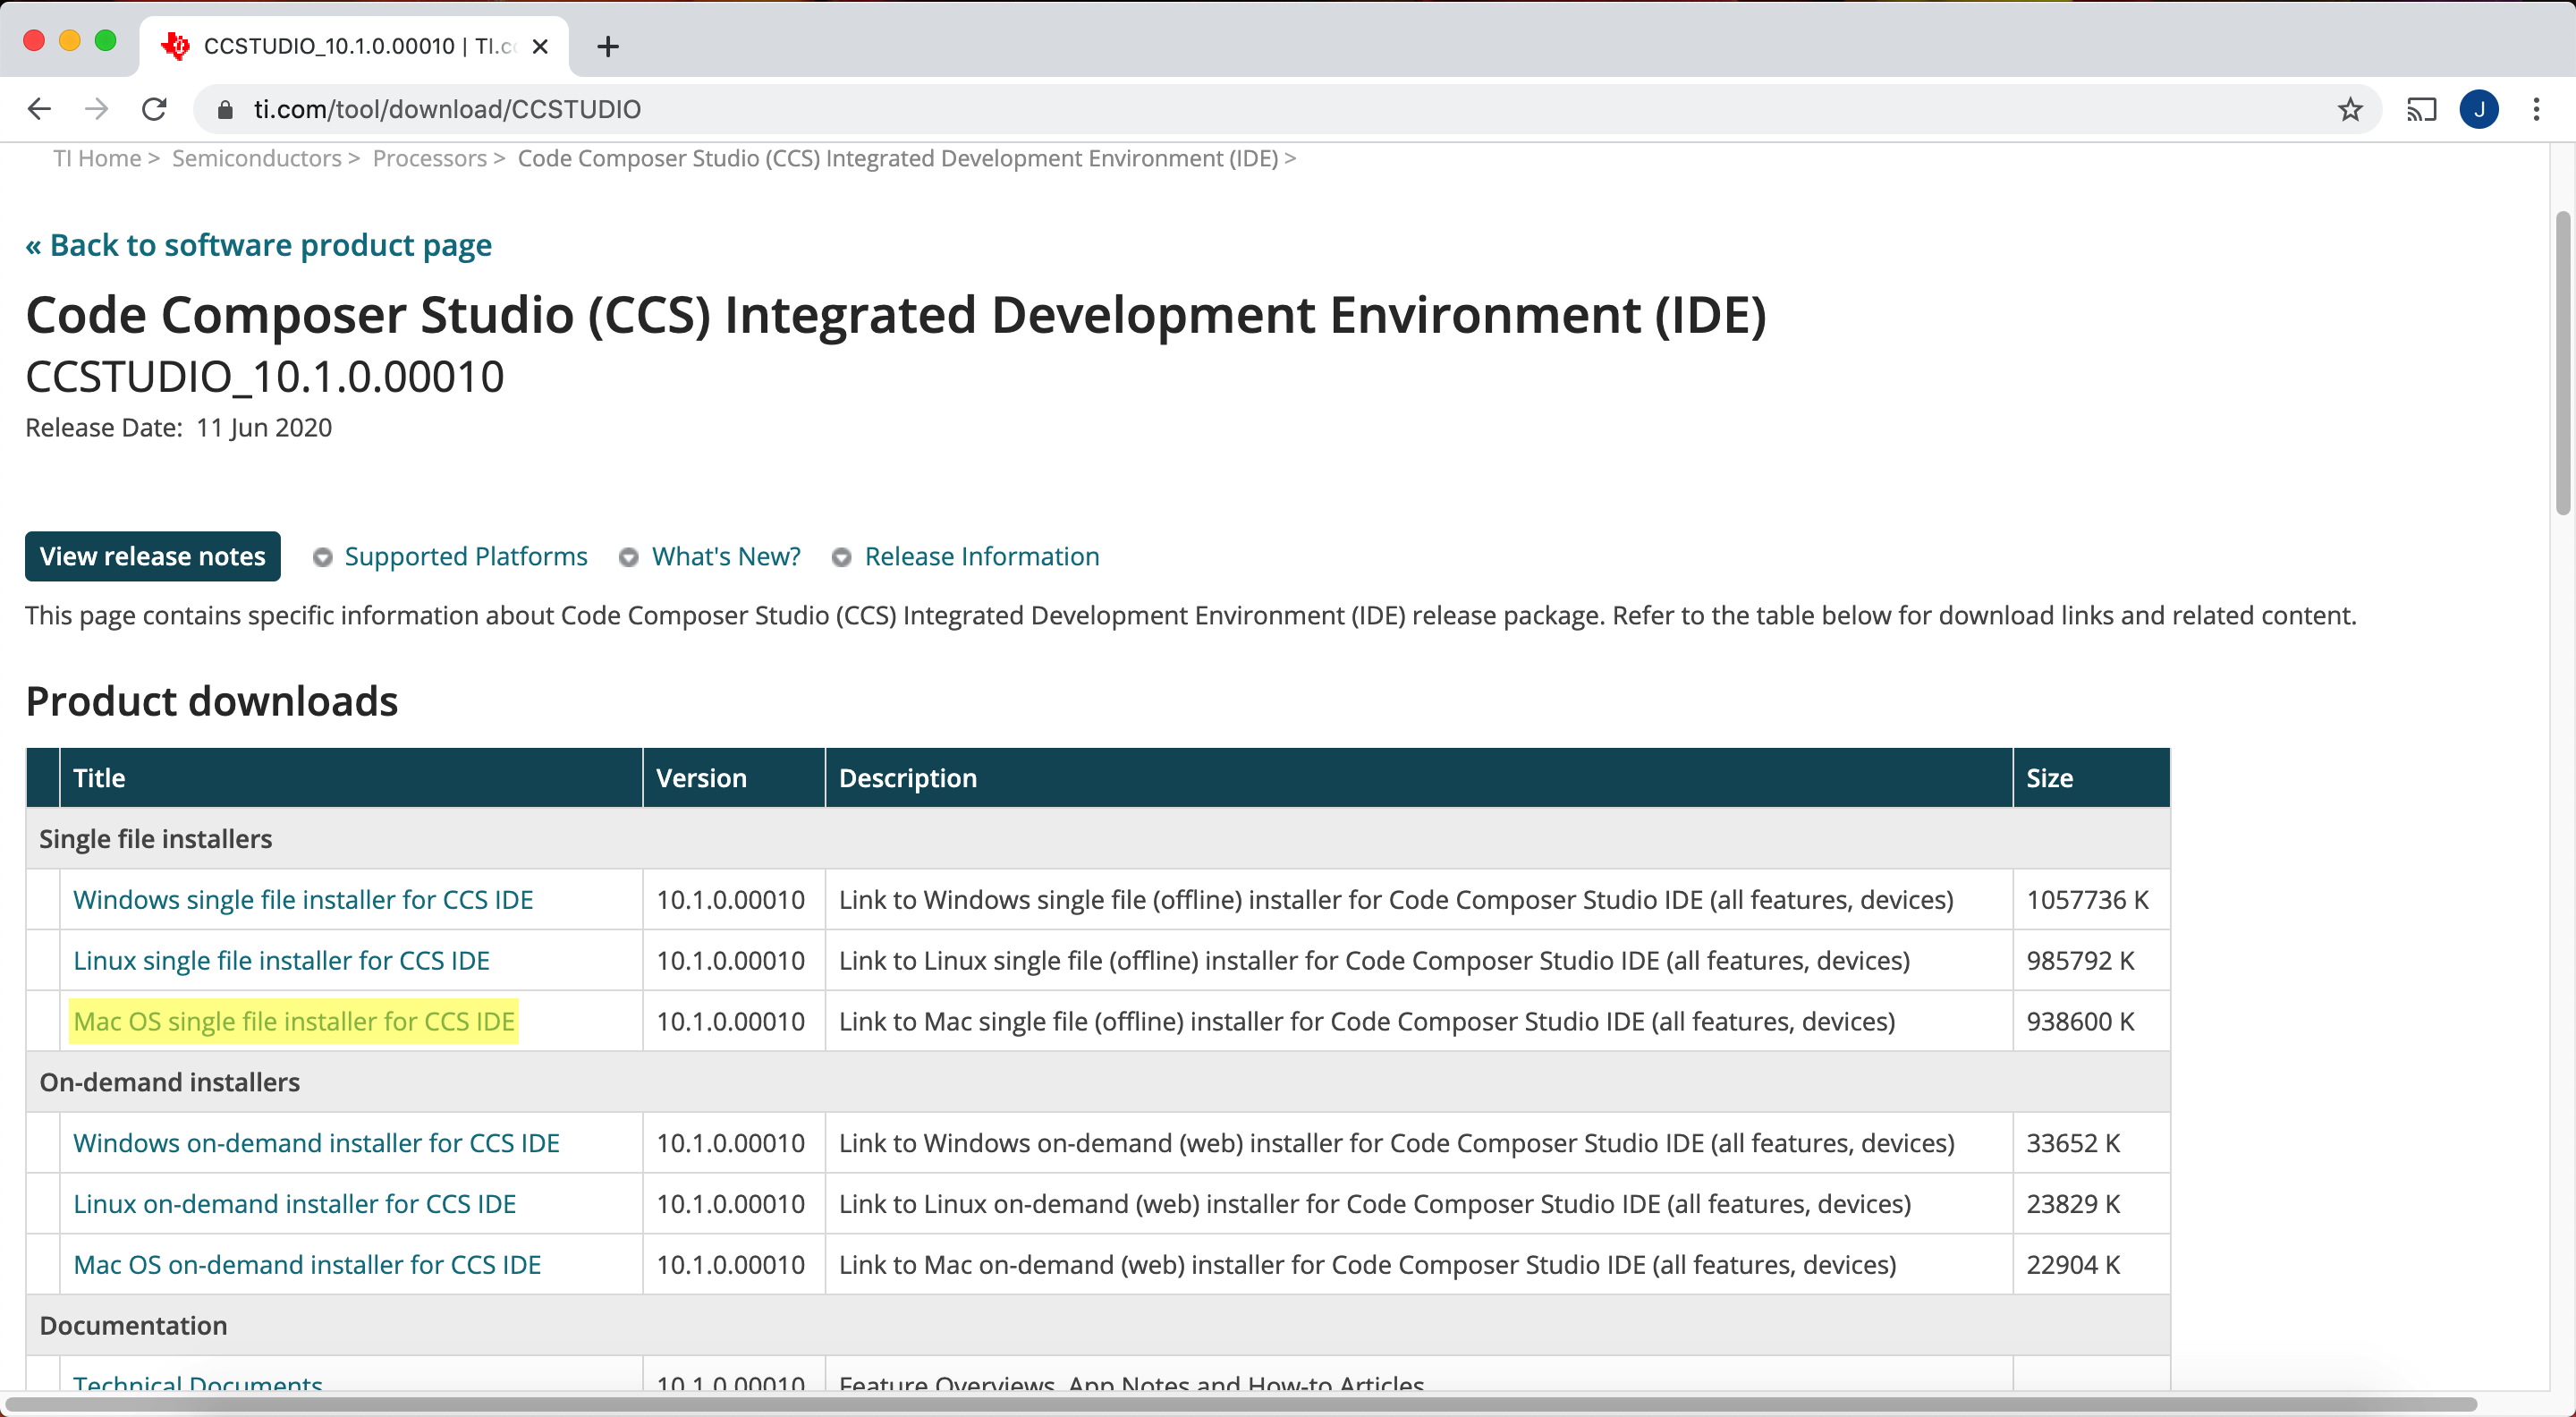
\includegraphics[width = 0.65\textwidth]{ccs_install_1} 
\end{figure}

Load the disk image and run the setup application:

\begin{figure}[H]
    \centering
  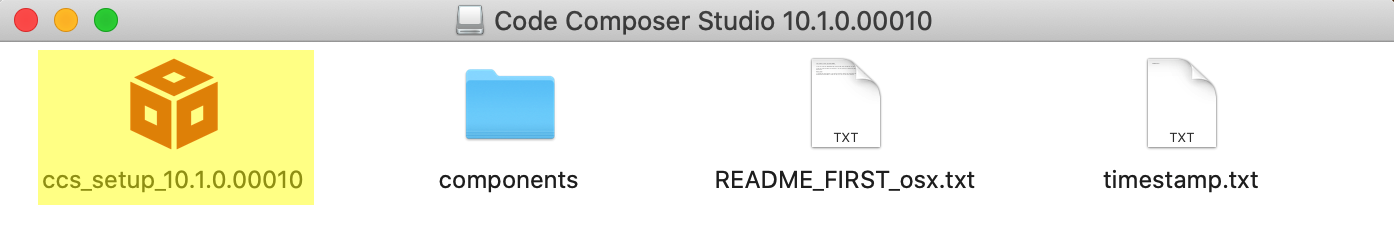
\includegraphics[width = 0.65\textwidth]{ccs_install_2} 
\end{figure}

In the installation setup, you can choose the full installation, but it is not necessary. If you choose the custom installation, the two necessary components are the MS430 ultra-low power MCUs and C2000 real-time MCUs. In the next window, select the additional debugger (SEGGER J-Link). (Note that the Mac doesn't have the Blackhawk Debug Probes available).

\begin{figure}[H]
    \centering
    {{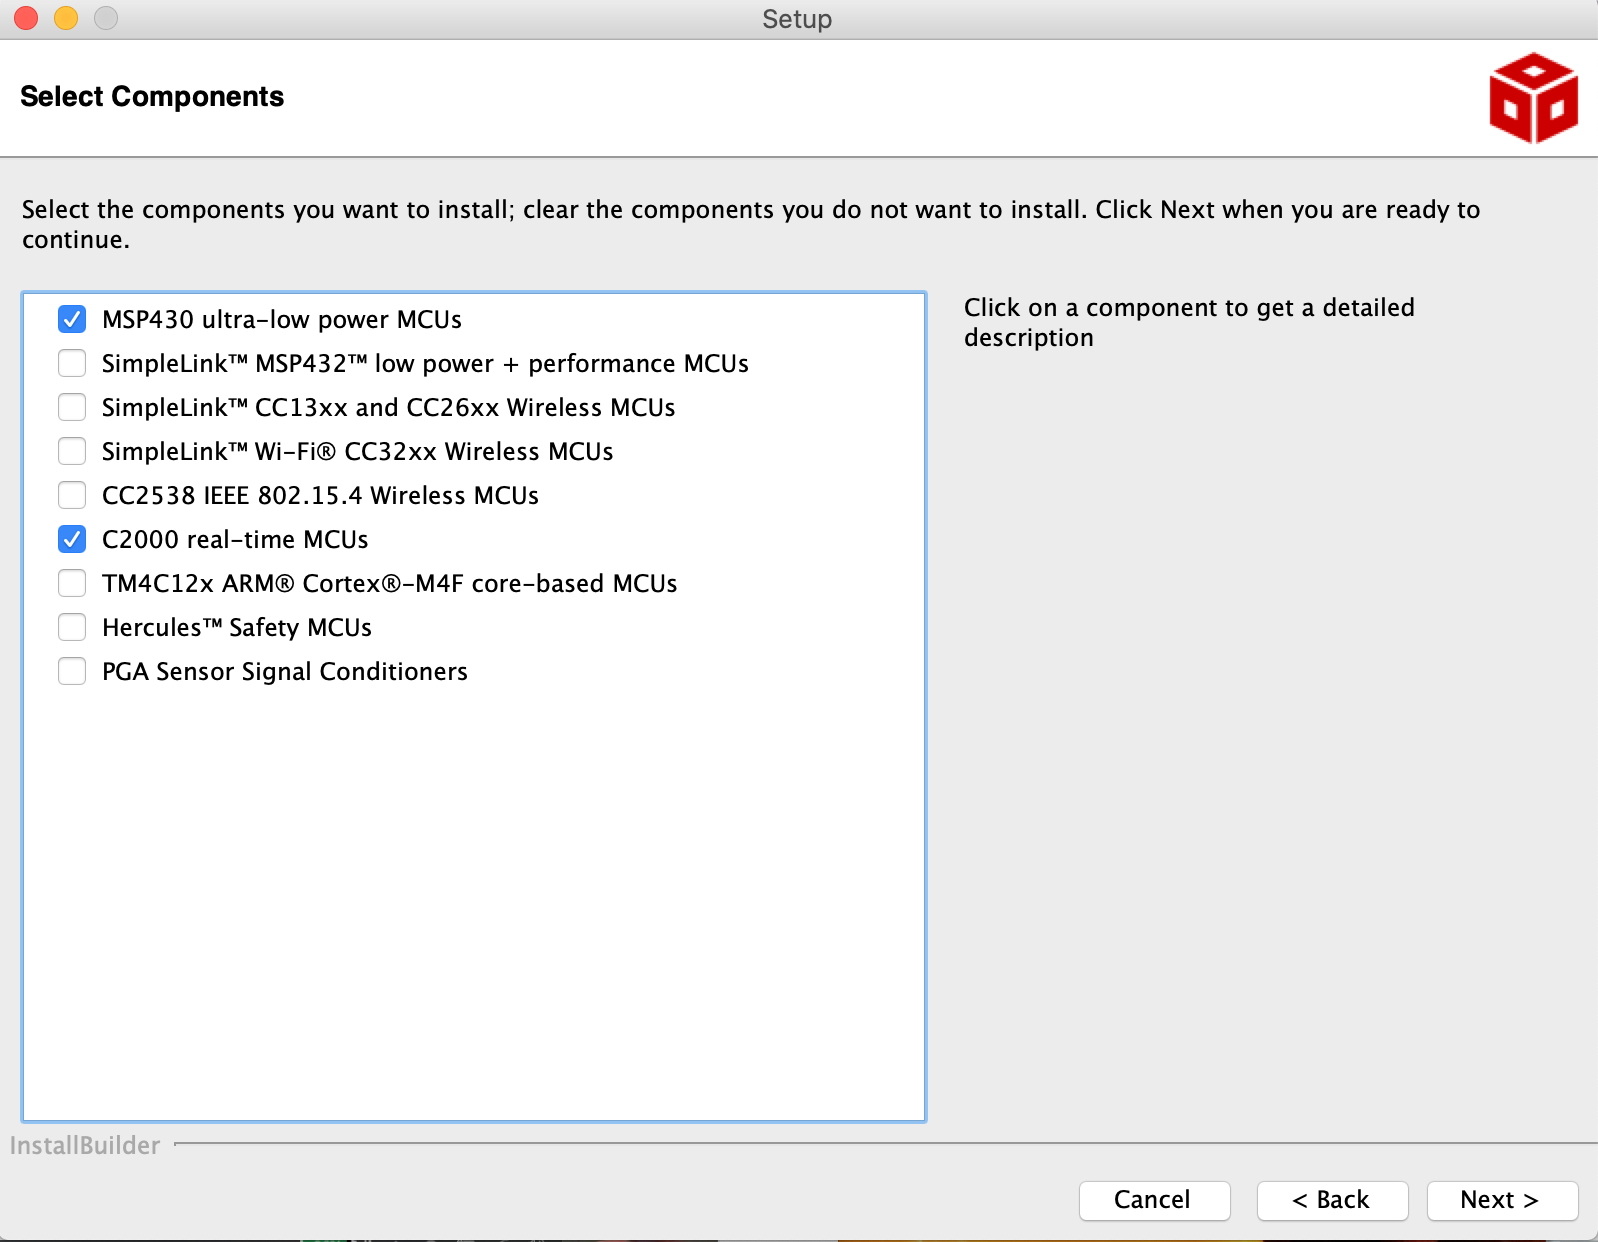
\includegraphics[width=0.325\textwidth]{ccs_install_3.png} }}
    \qquad
    {{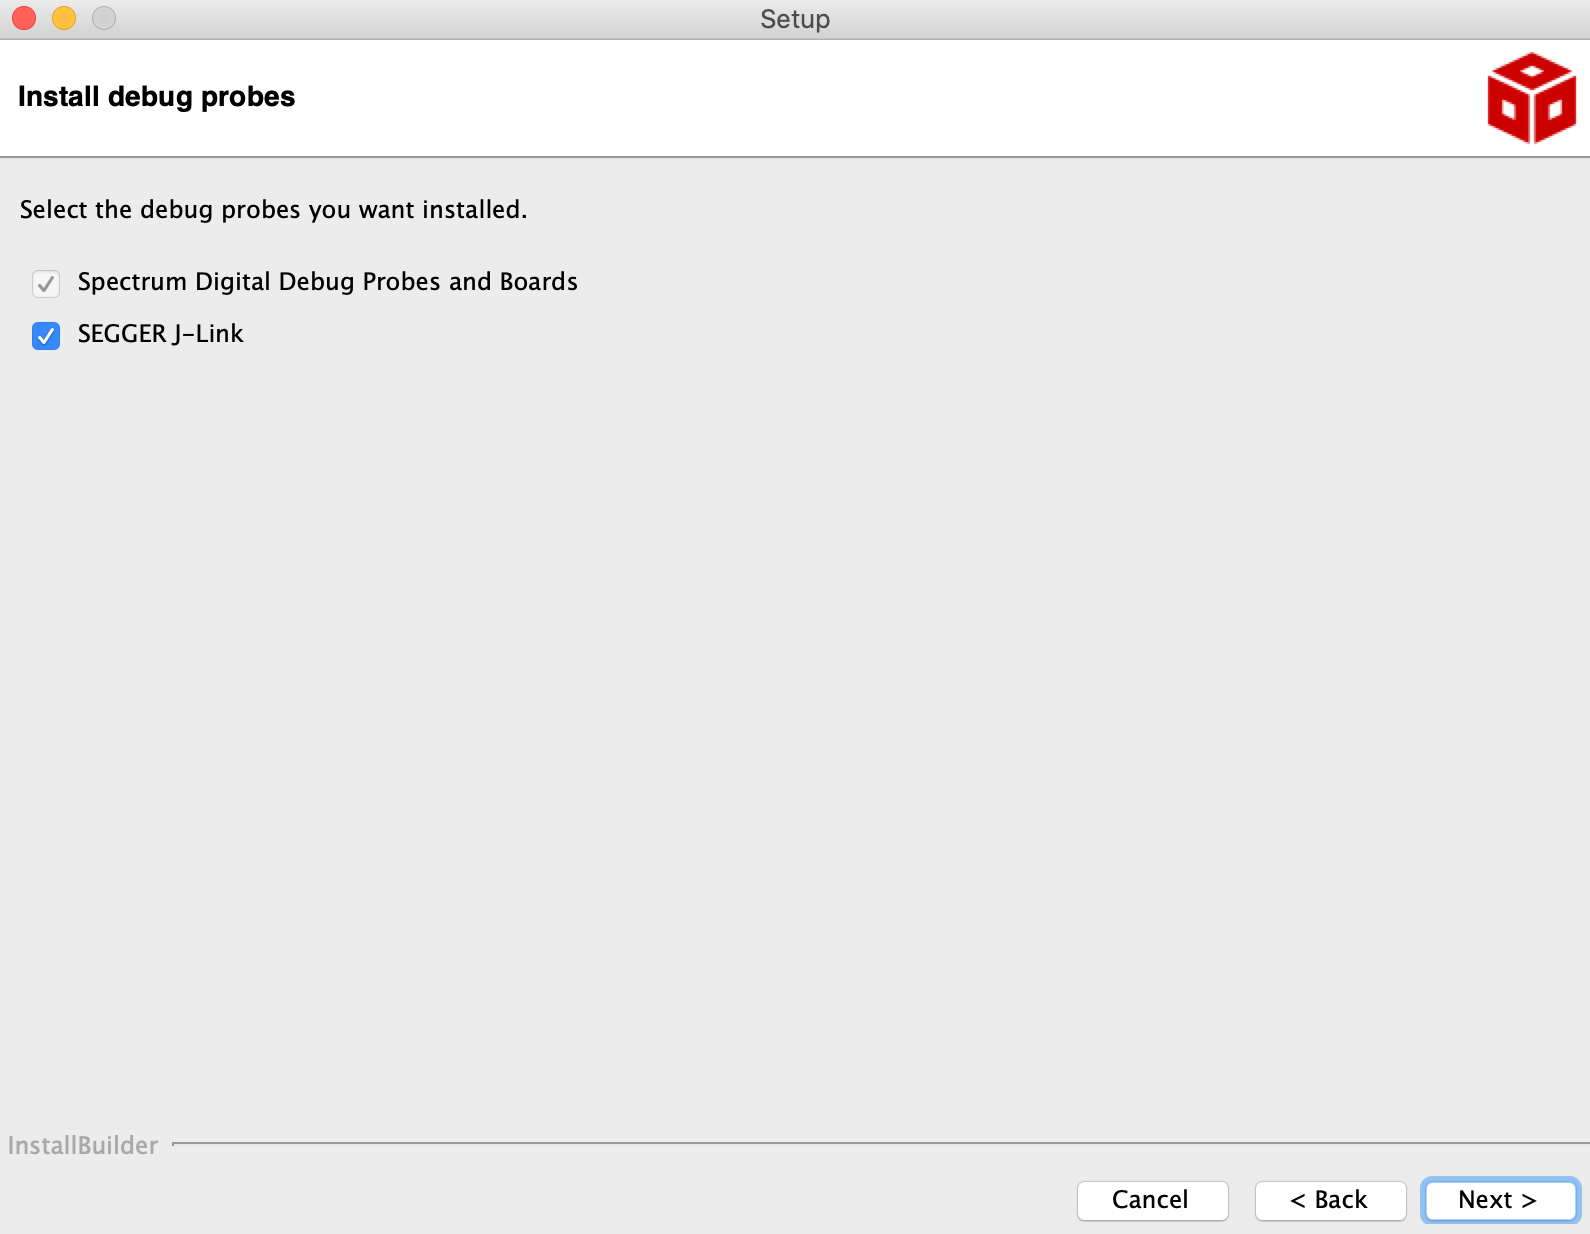
\includegraphics[width=0.325\textwidth]{ccs_install_4.png} }}
\end{figure}

Installation is now complete (note that the installer will also install Eclipse).

\pagebreak

\subsection{CCS Configuration}

When launching CCS for the first time, you will need to install the CCS2000 software. Do this by navigating to the resource explorer, software folder and C2000Ware. Click install to complete.

\begin{figure}[H]
    \centering
    {{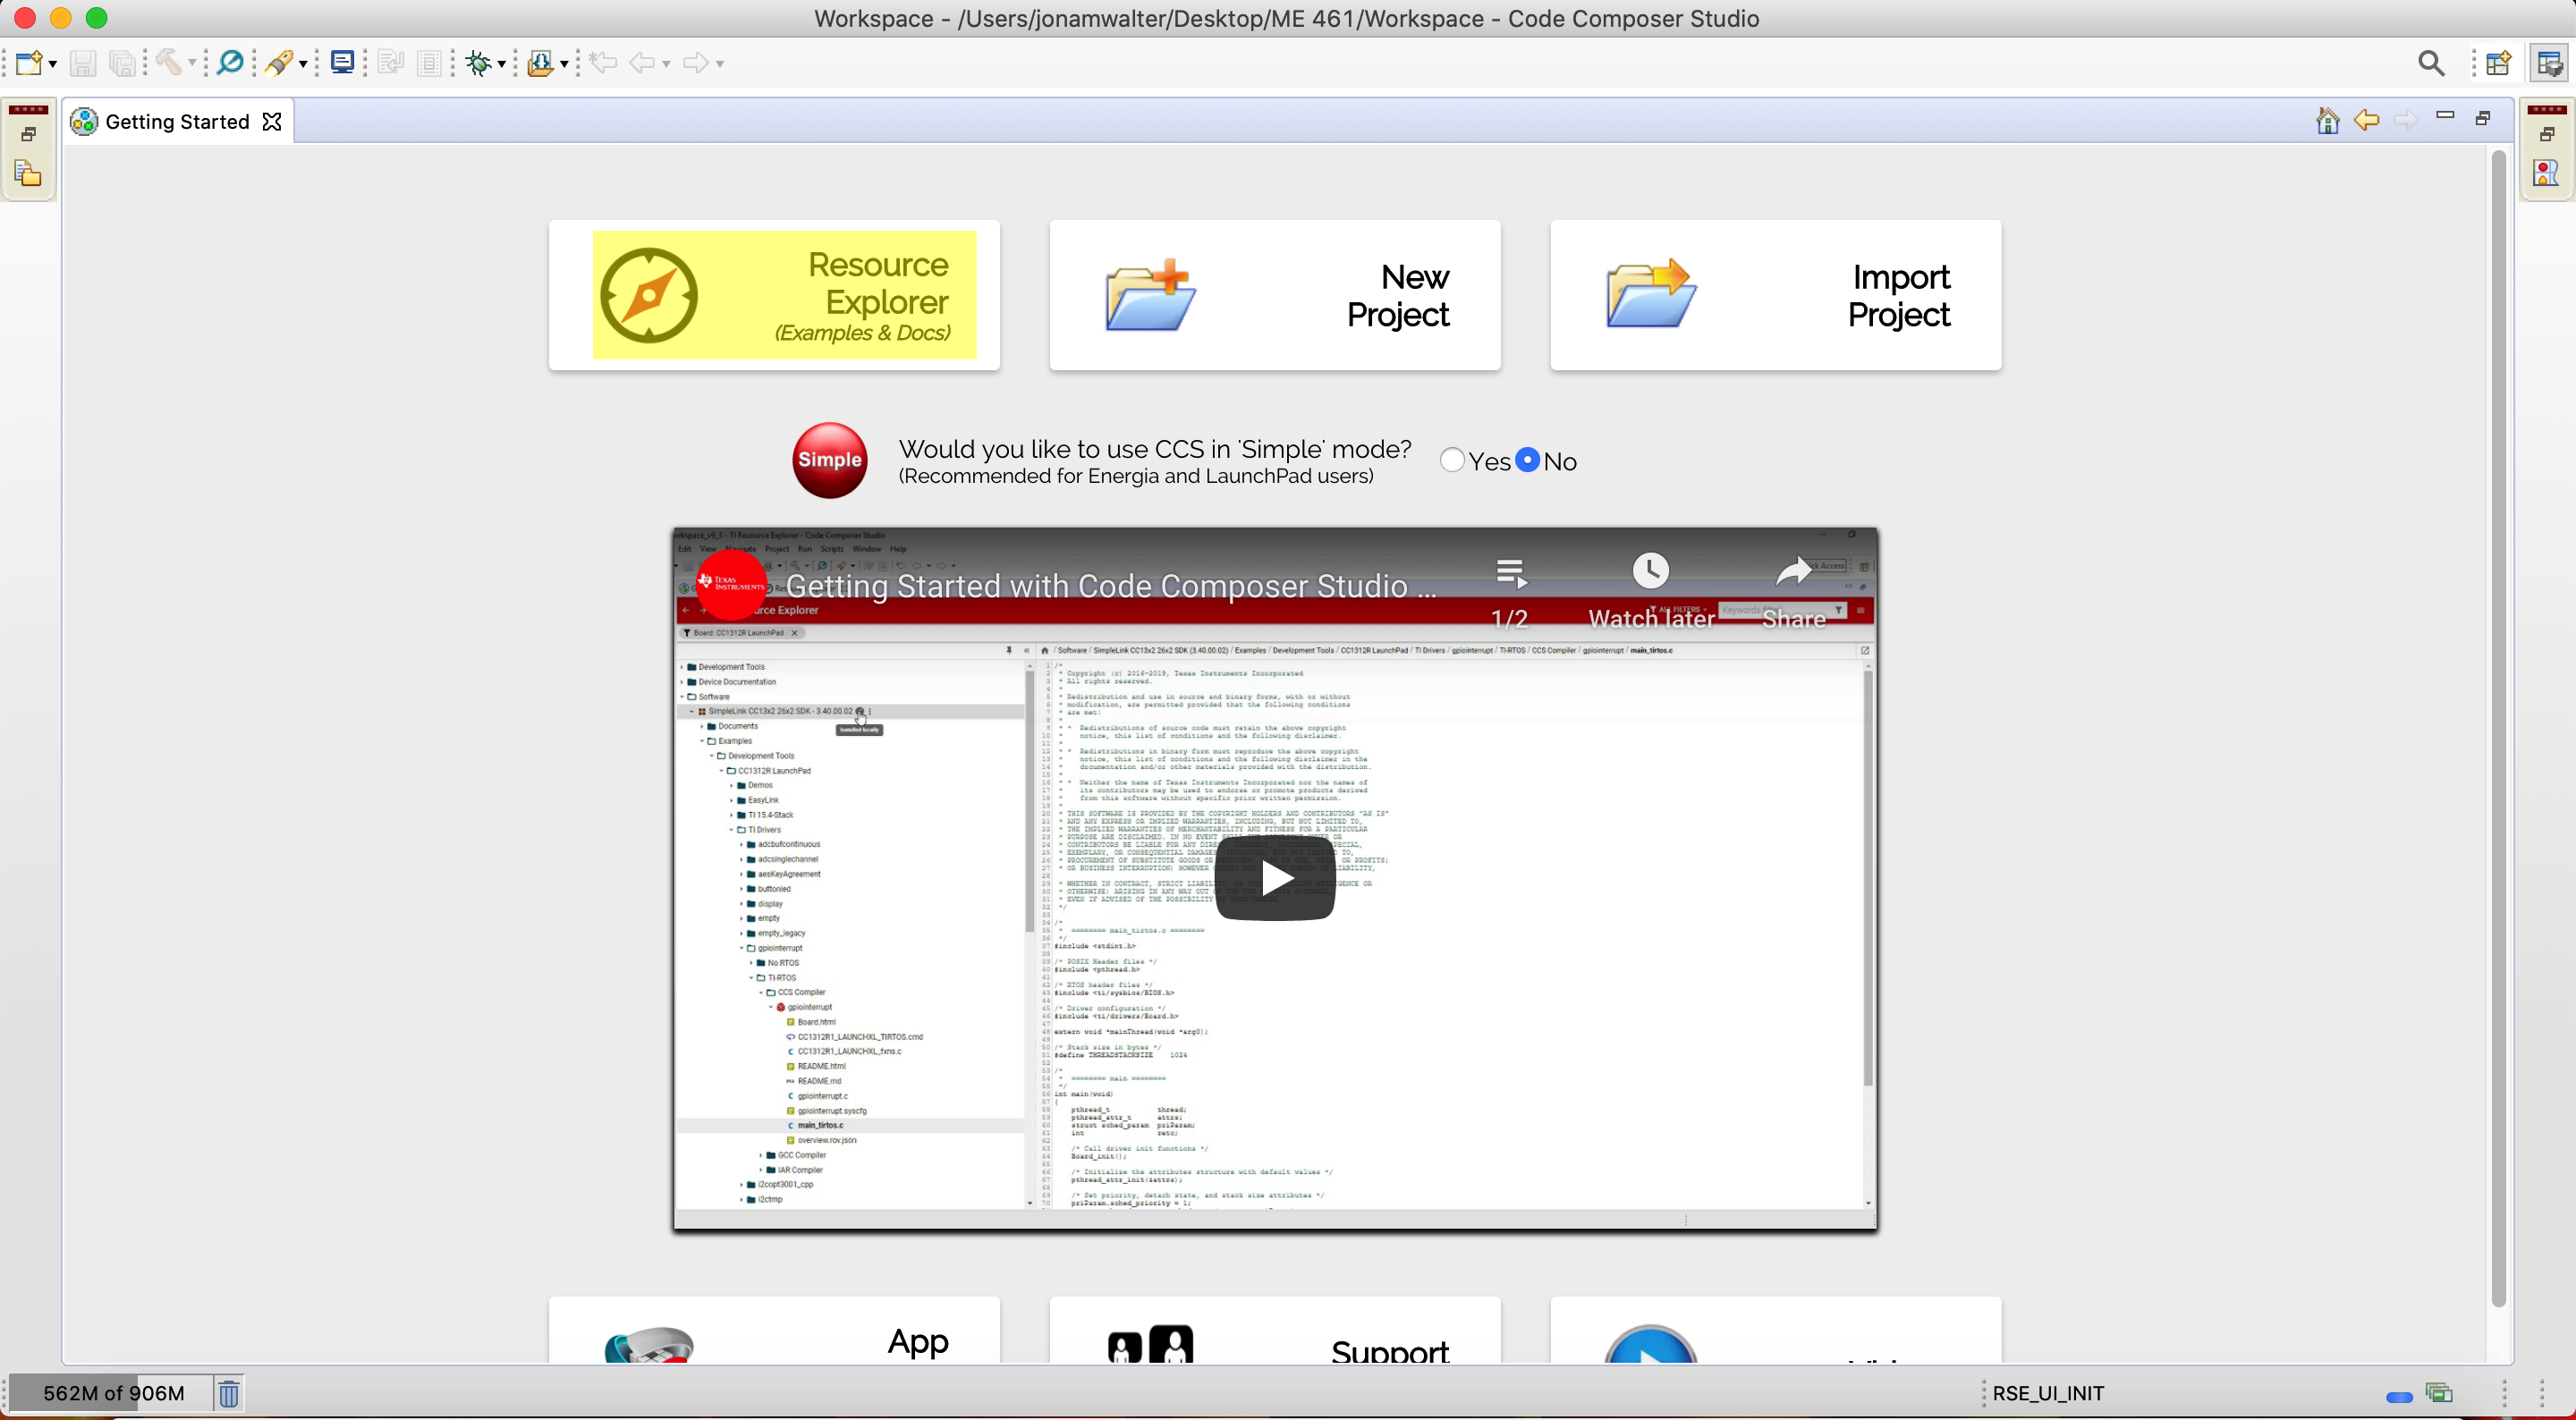
\includegraphics[width=0.5\textwidth]{ccs_configure_1.png} }}
    \qquad
    {{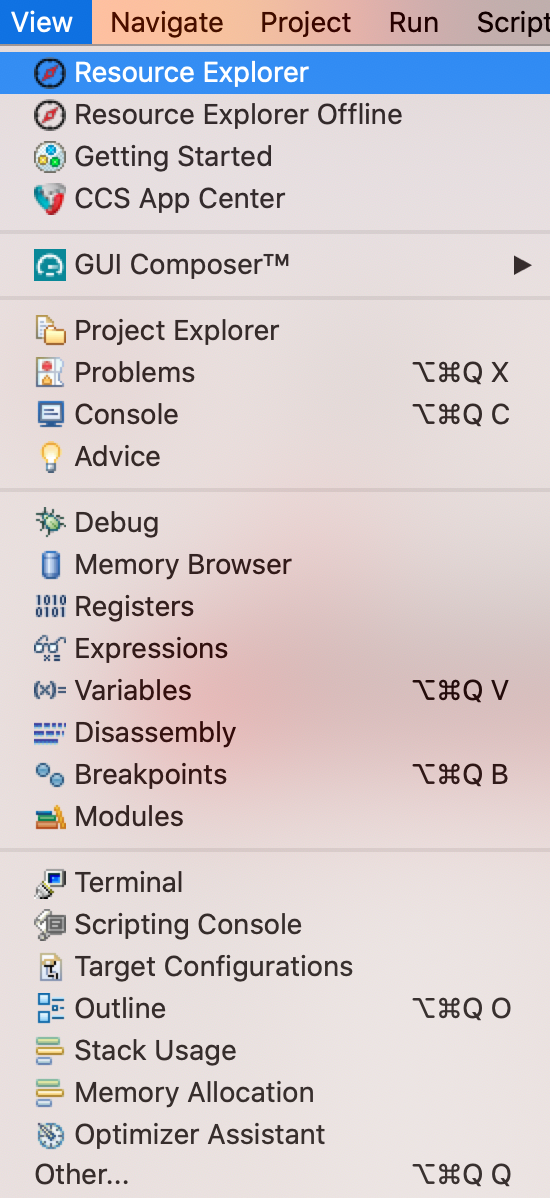
\includegraphics[width=0.15\textwidth]{ccs_configure_2.png} }}
\end{figure}

\begin{figure}[H]
    \centering
  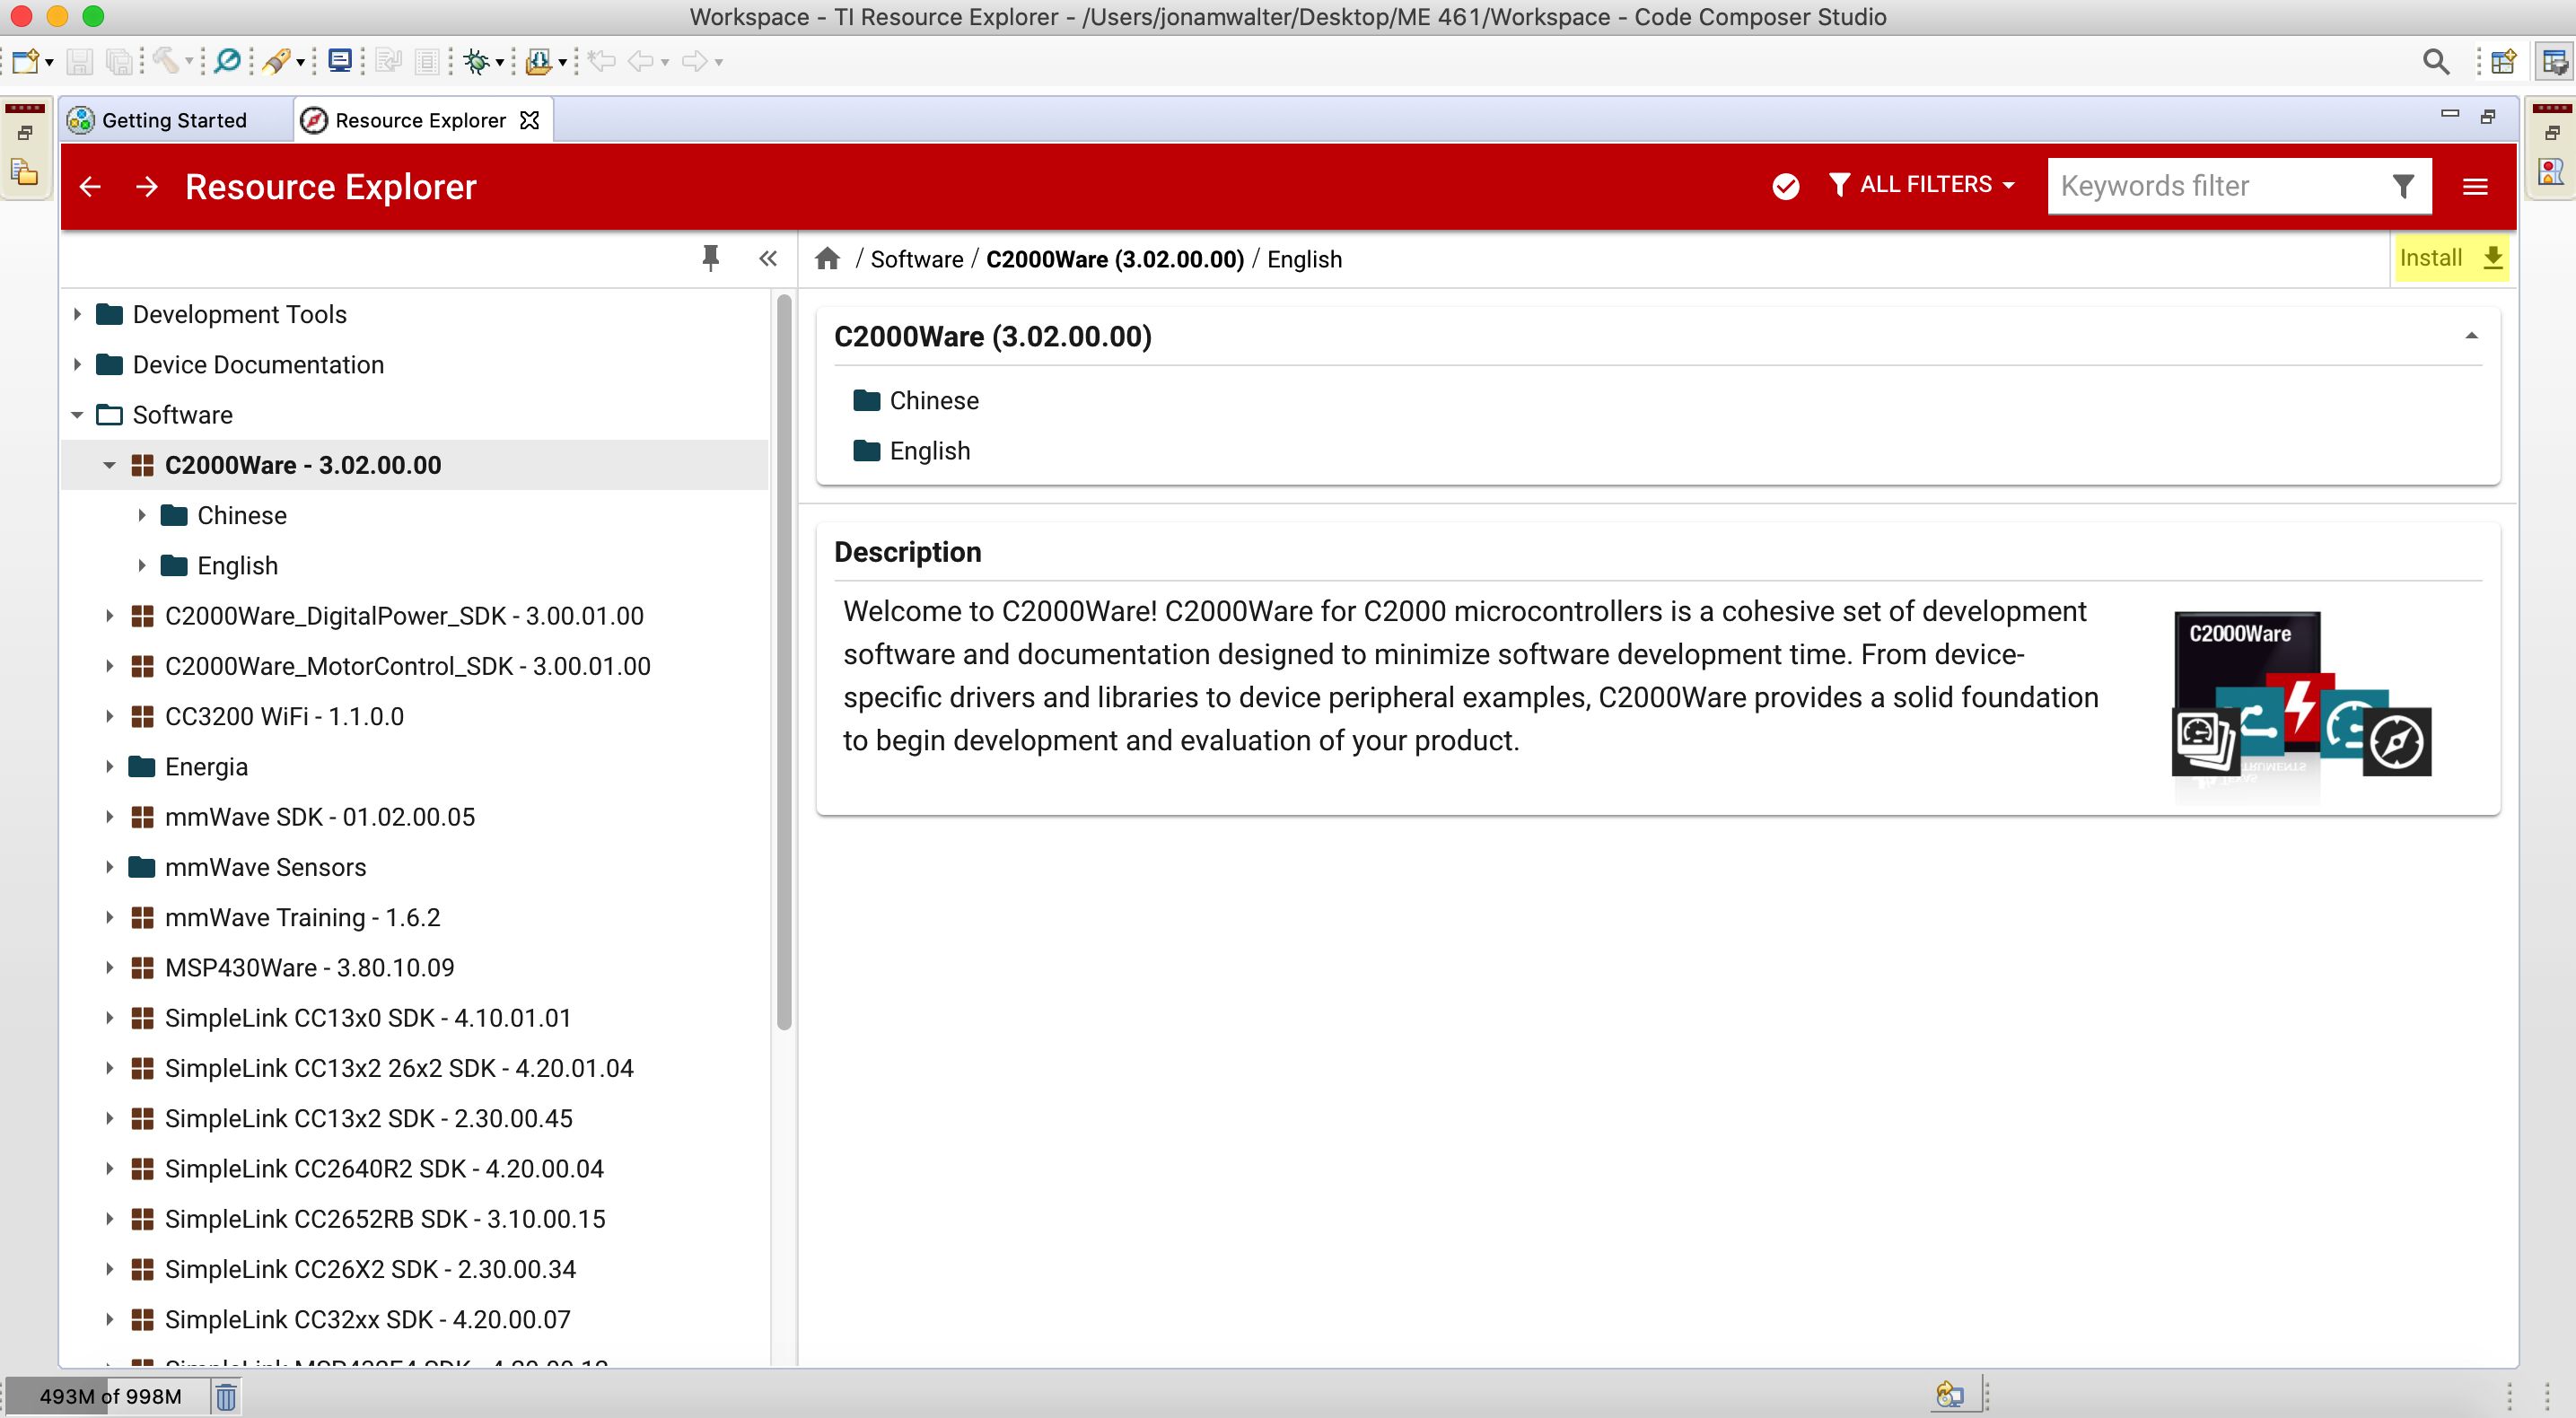
\includegraphics[width = 0.65\textwidth]{ccs_configure_3.png} 
\end{figure}

You can check the progress of the install by clicking on the clock:

\begin{figure}[H]
    \centering
  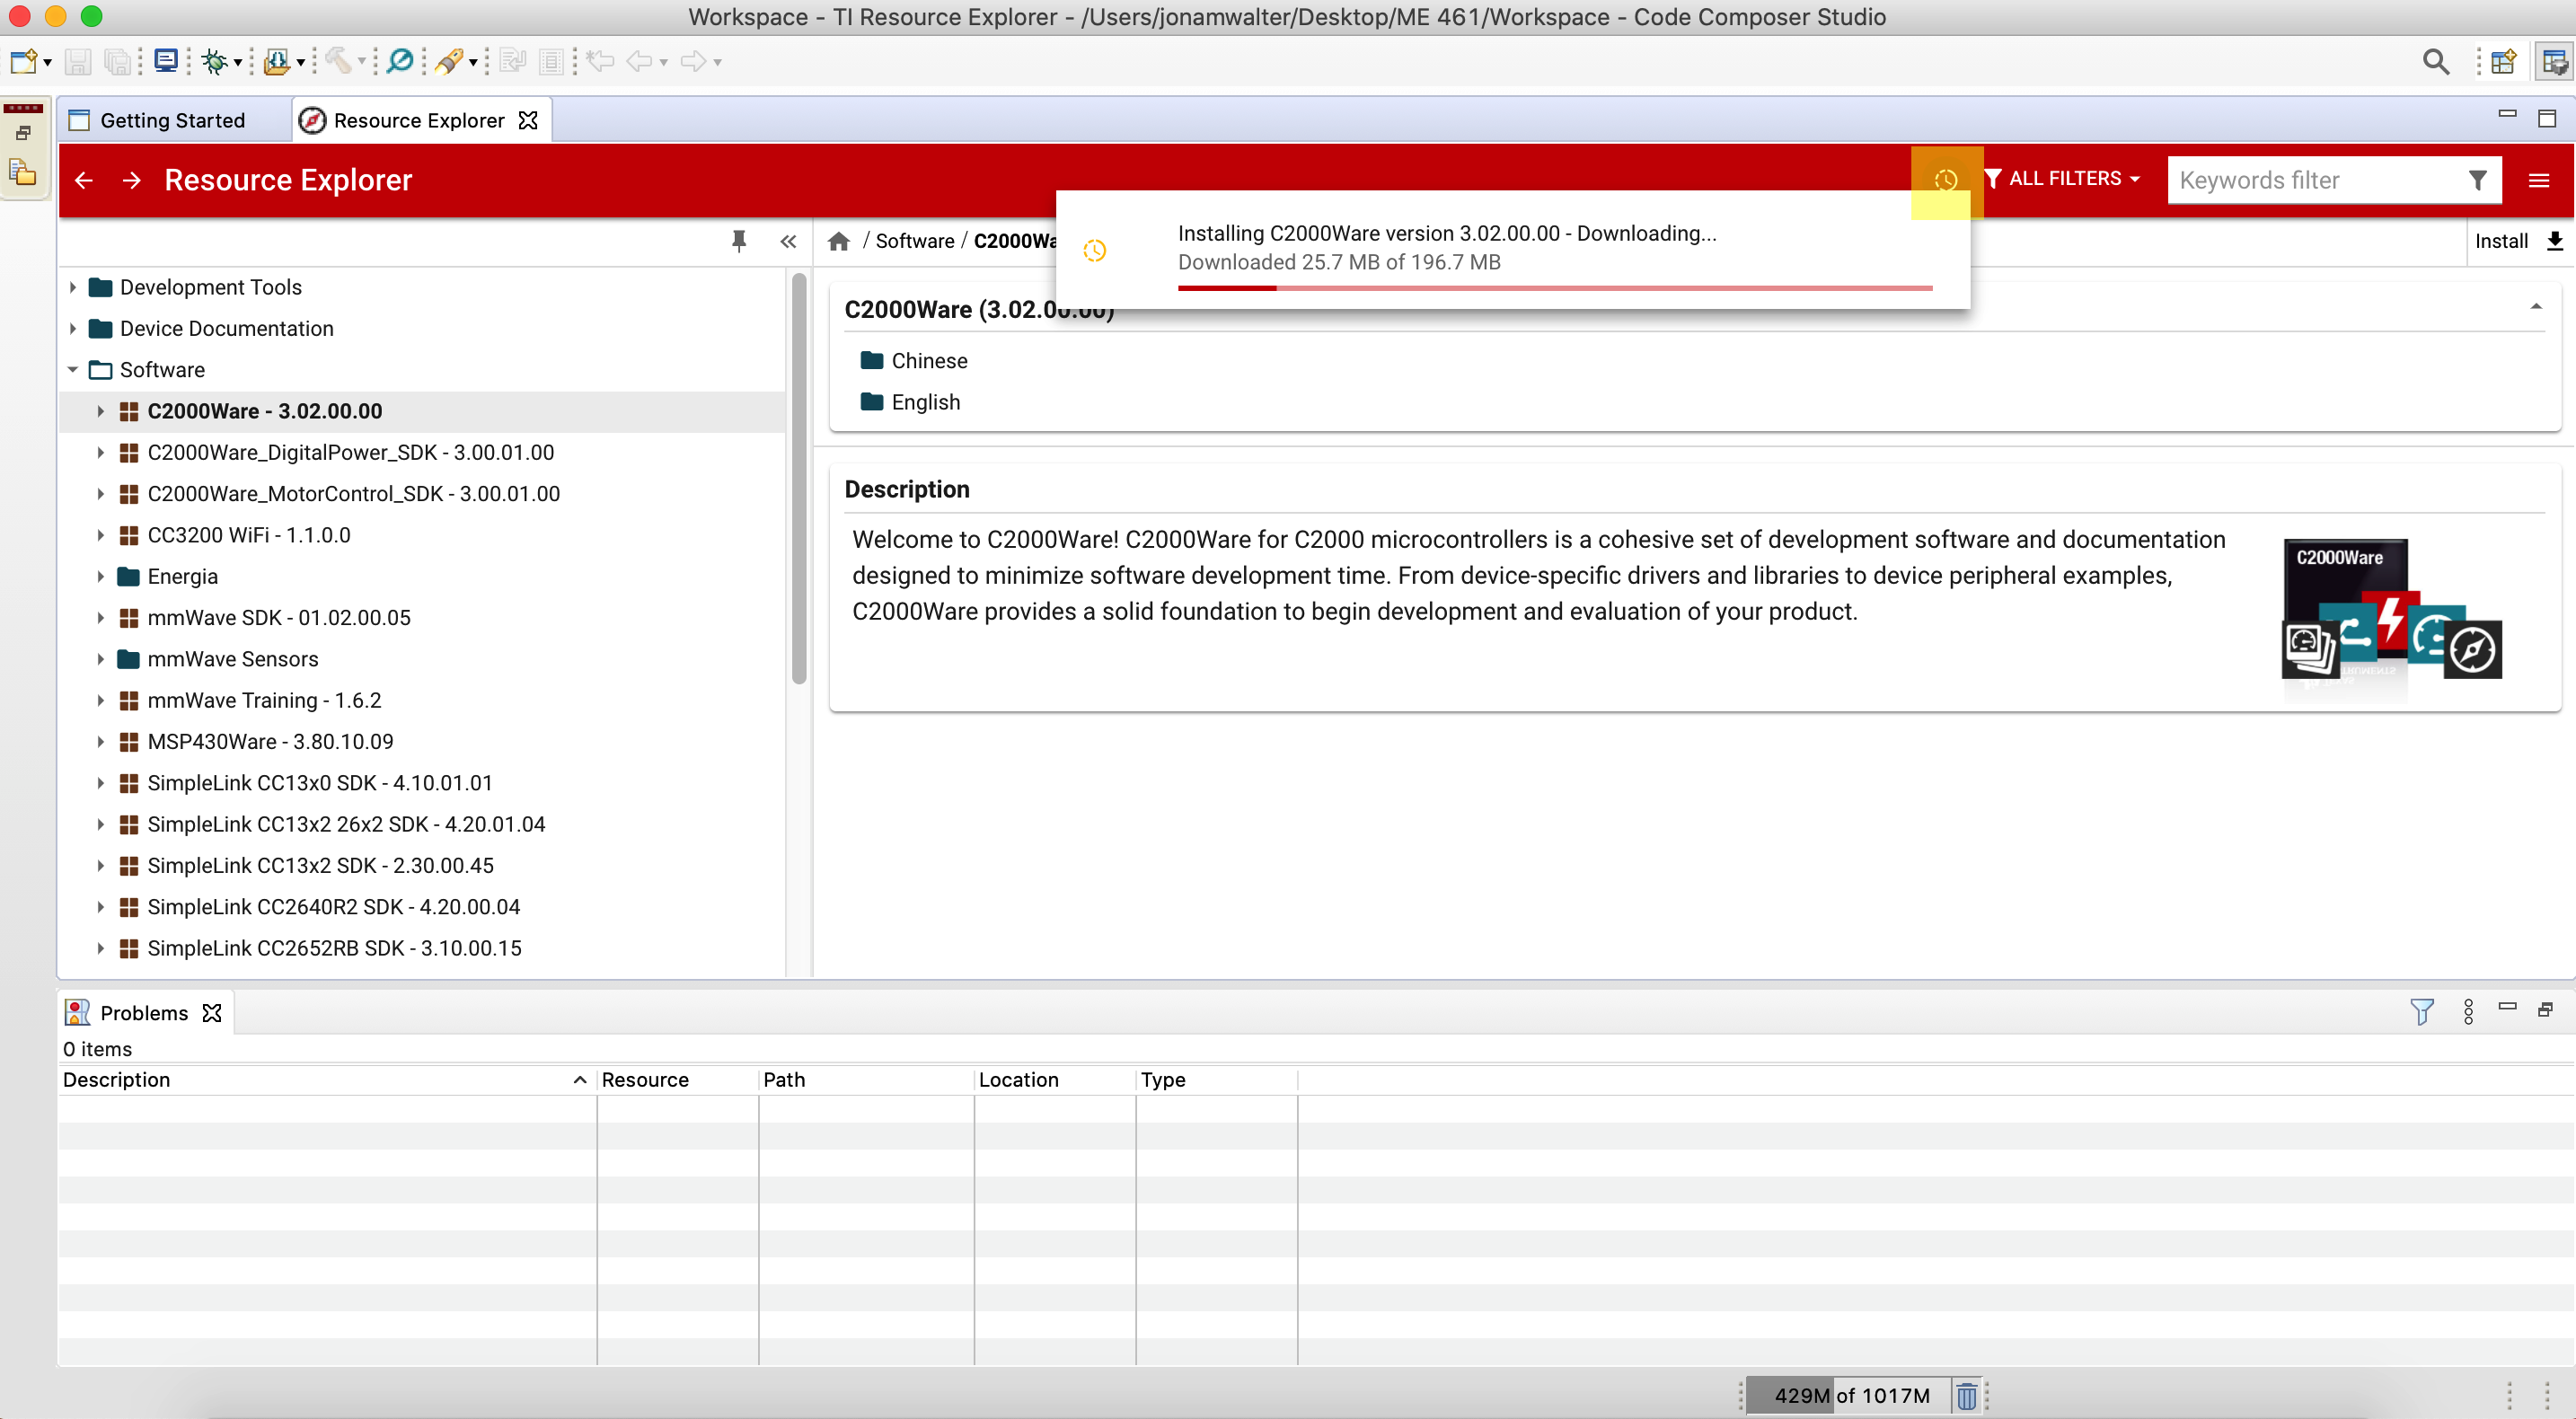
\includegraphics[width = 0.65\textwidth]{ccs_configure_4} 
\end{figure}

\subsection{Workspaces}

When you first open CCS it asks you to choose a directory for the current workspace. The workspace is the main working folder and has the information to manage all the projects assigned to it.

\begin{figure}[H]
    \centering
    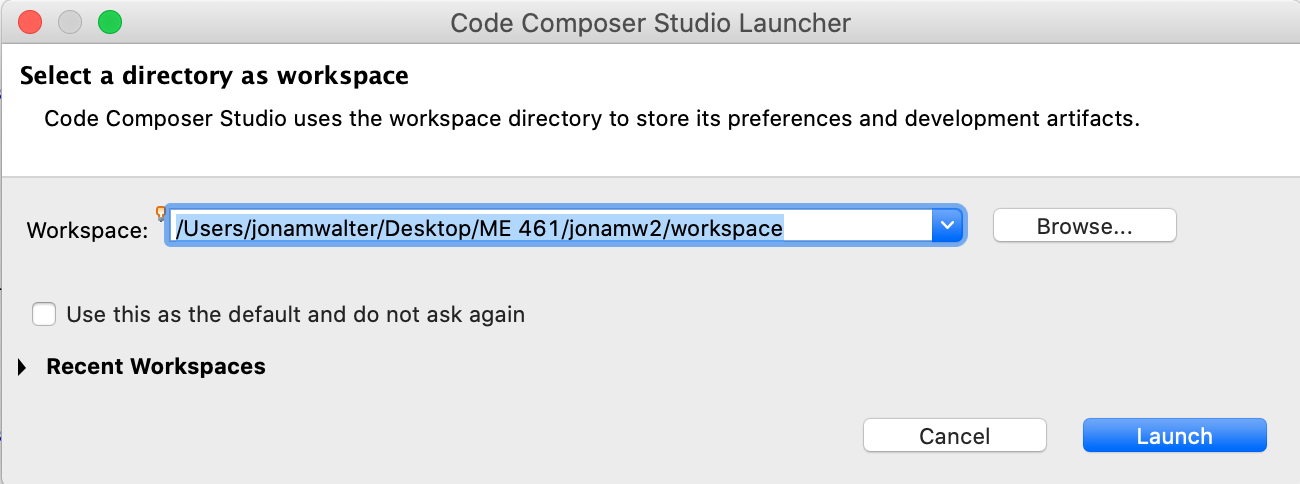
\includegraphics[width = 0.4\textwidth]{ccs_workspaces_1} 
\end{figure}

If the workspace prompt is disabled, navigate to Code Composer Studio$\rightarrow$Preferences, search for prompt, change the setting, click apply and close.

\begin{figure}[H]
    \centering
    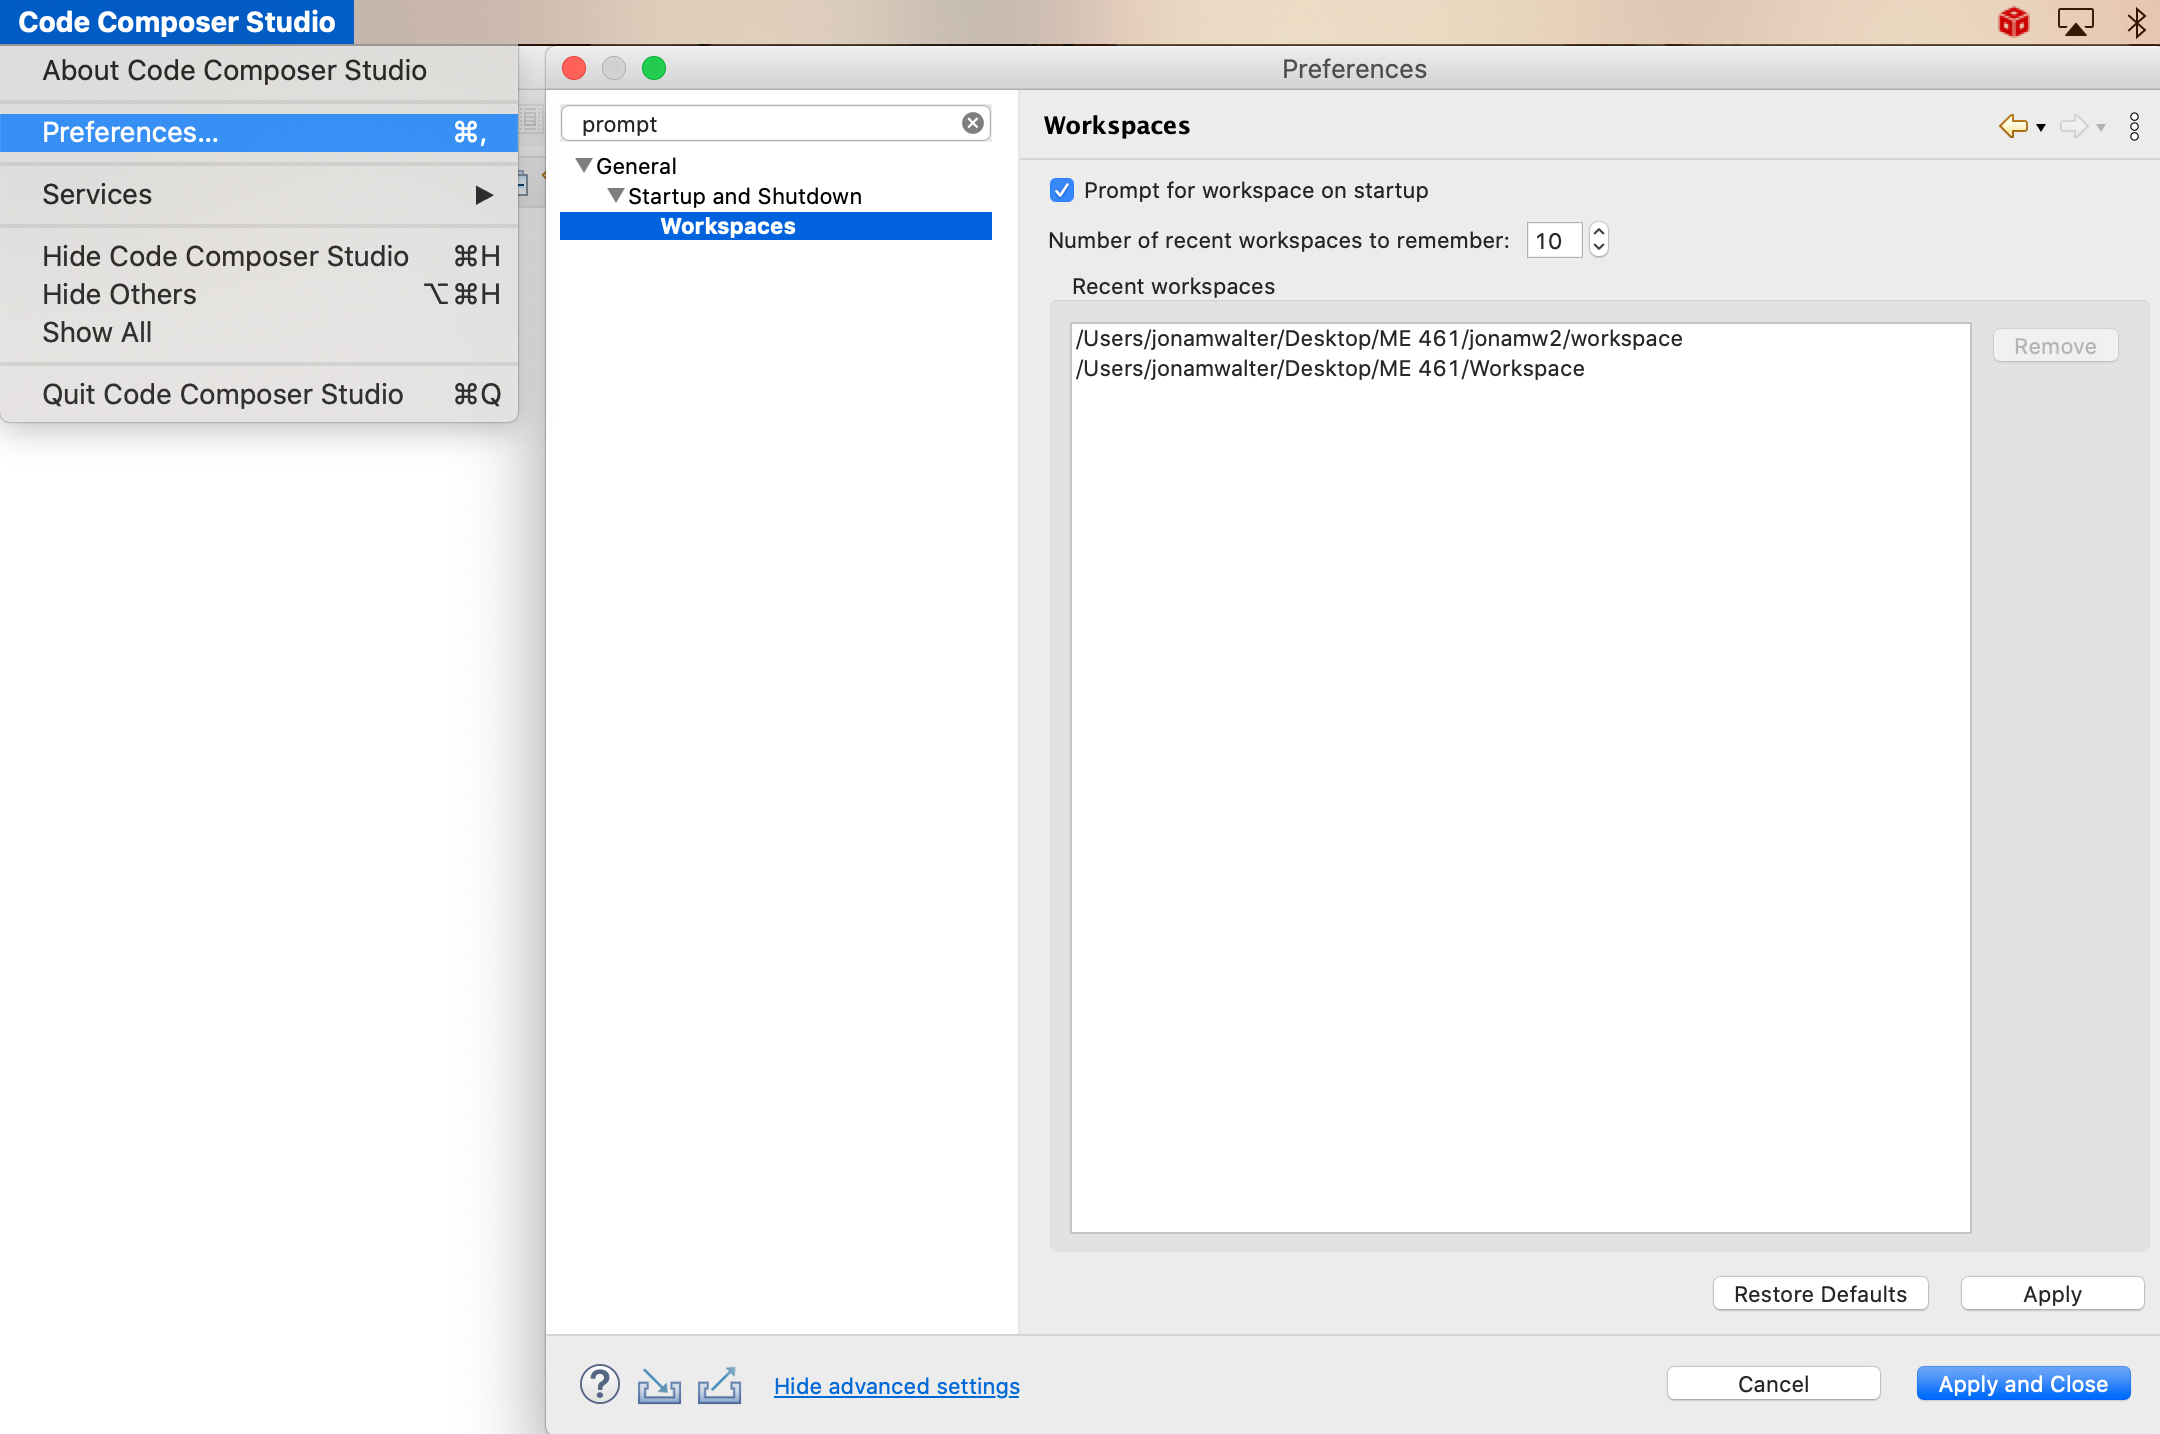
\includegraphics[width = 0.4\textwidth]{ccs_workspaces_2} 
\end{figure}

\pagebreak

\subsection{Projects}

Projects are places in your workspace that are collections of files to run code. To start a new project navigate to file$\rightarrow$import to open and choose the appropriate import wizard:

\begin{figure}[H]
    \centering
  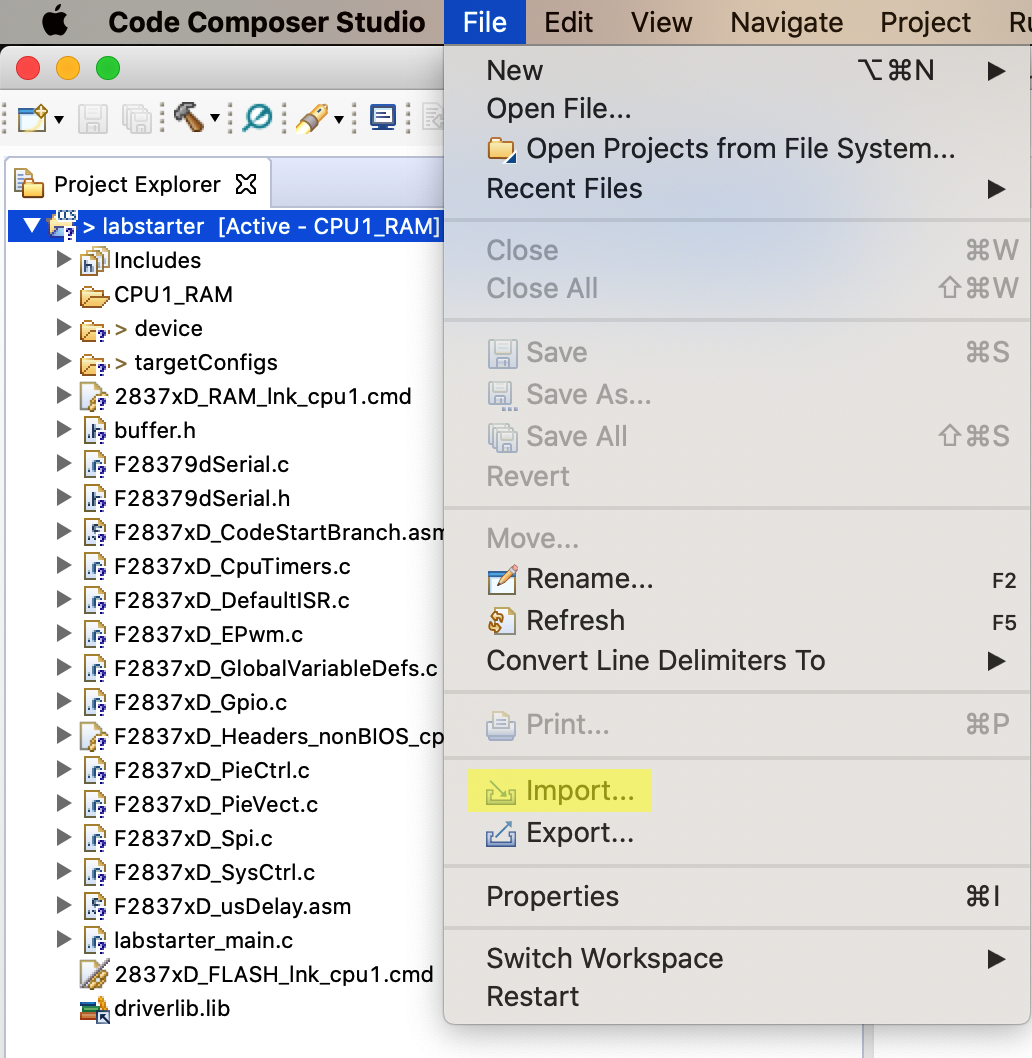
\includegraphics[width = 0.3\textwidth]{ccs_projects_1} 
  \qquad
    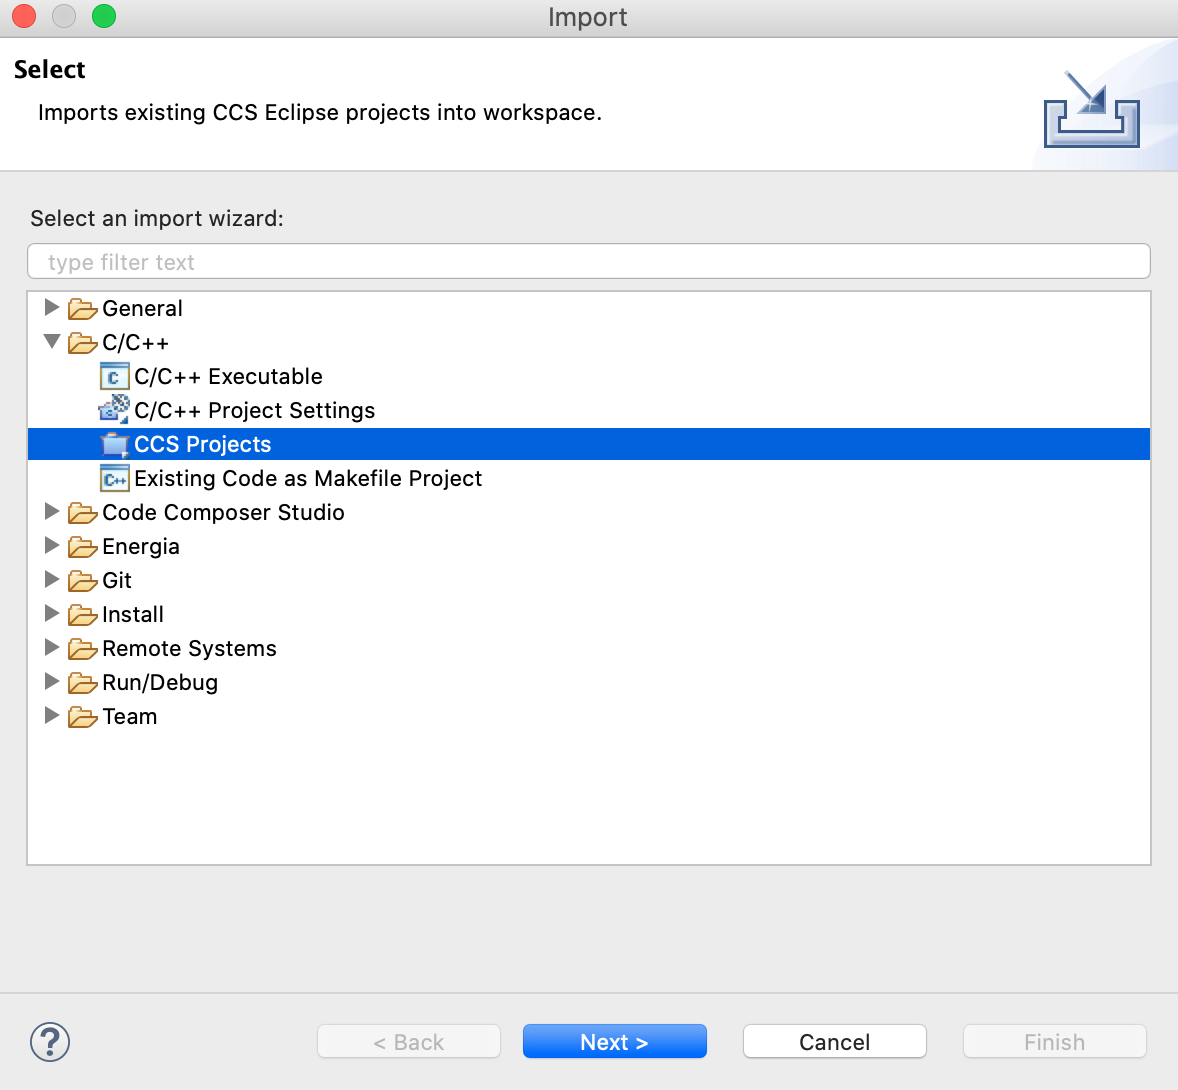
\includegraphics[width = 0.3\textwidth]{ccs_projects_2} 
\end{figure}

Browse for the desired project folder and open the project:

\begin{figure}[H]
    \centering
  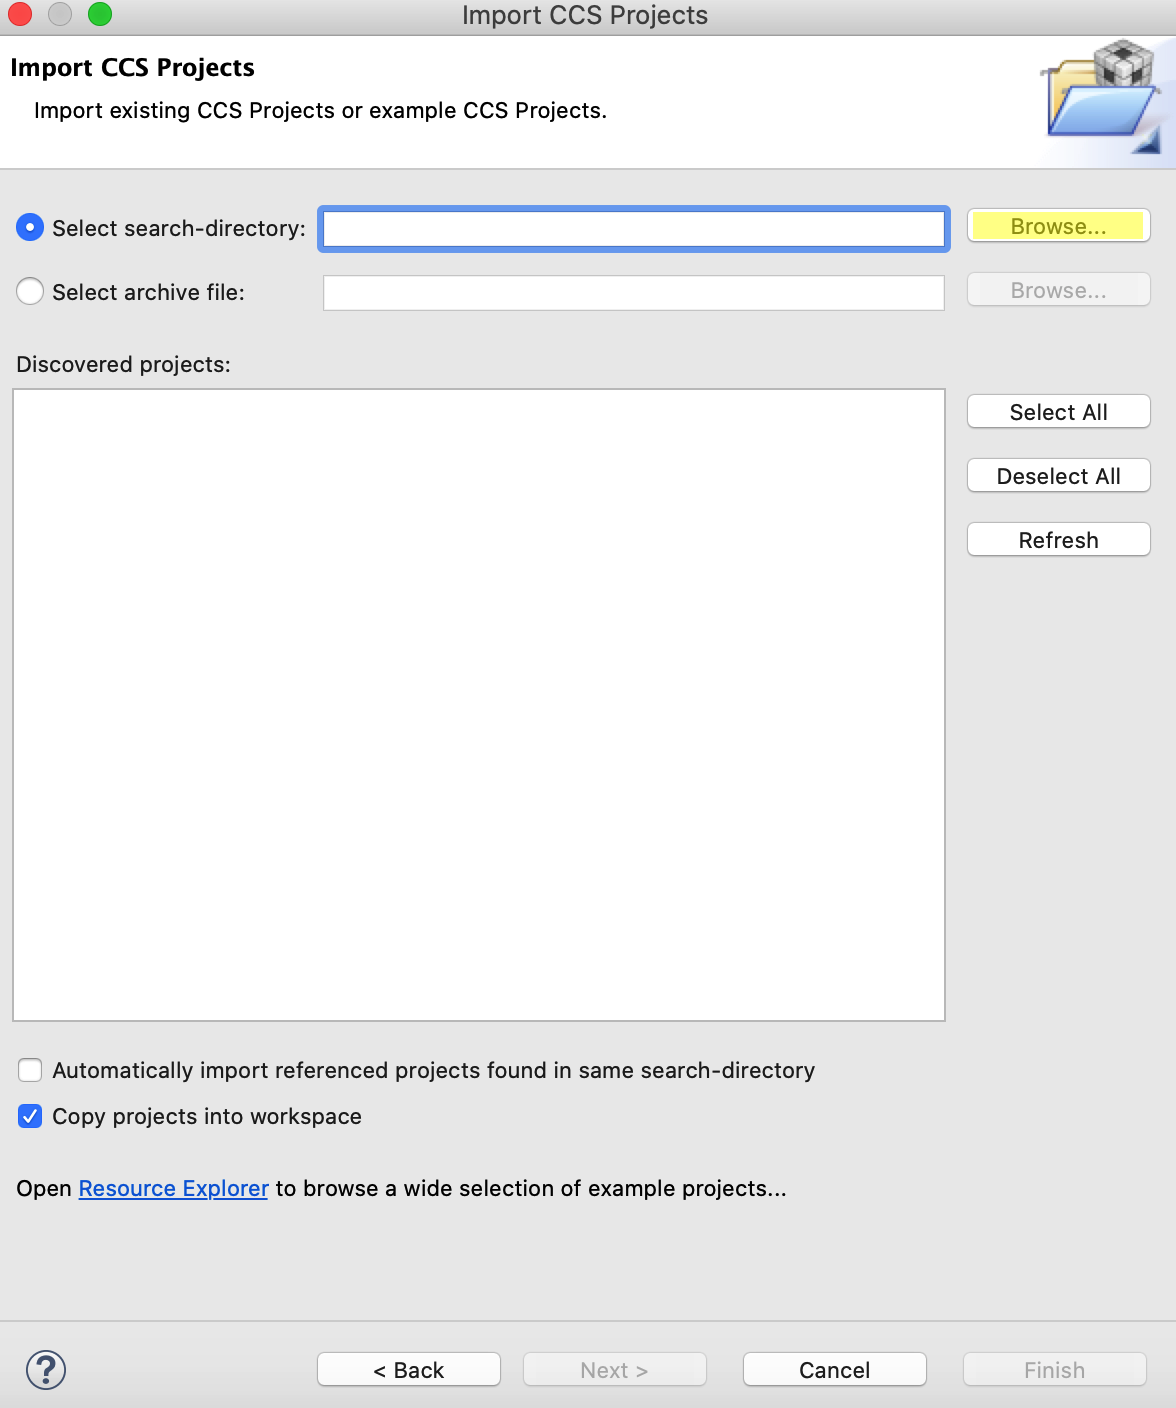
\includegraphics[width = 0.3\textwidth]{ccs_projects_3} 
\end{figure}

\pagebreak

\subsection{Errors}

If you get an error message similar to:

\verb|unable to launch CCS debug-session , The specified file C:\\...\\|

\verb|TMS320F28027_xd100v2.ccxml does not exist in the file systems|

when trying to run a project for the first time, right click the project, open properties and set the connection.

\begin{figure}[H]
    \centering
  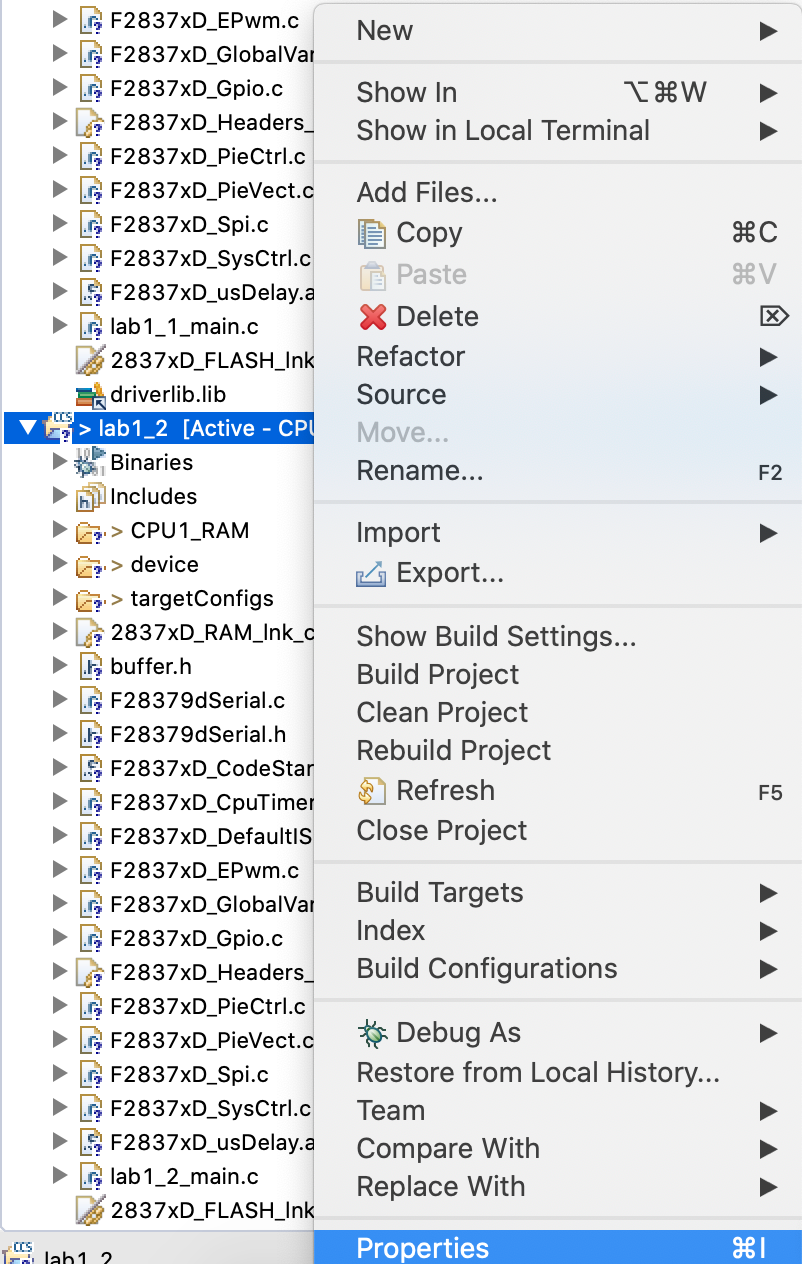
\includegraphics[width = 0.25\textwidth]{ccs_errors_1.png}
  \qquad
  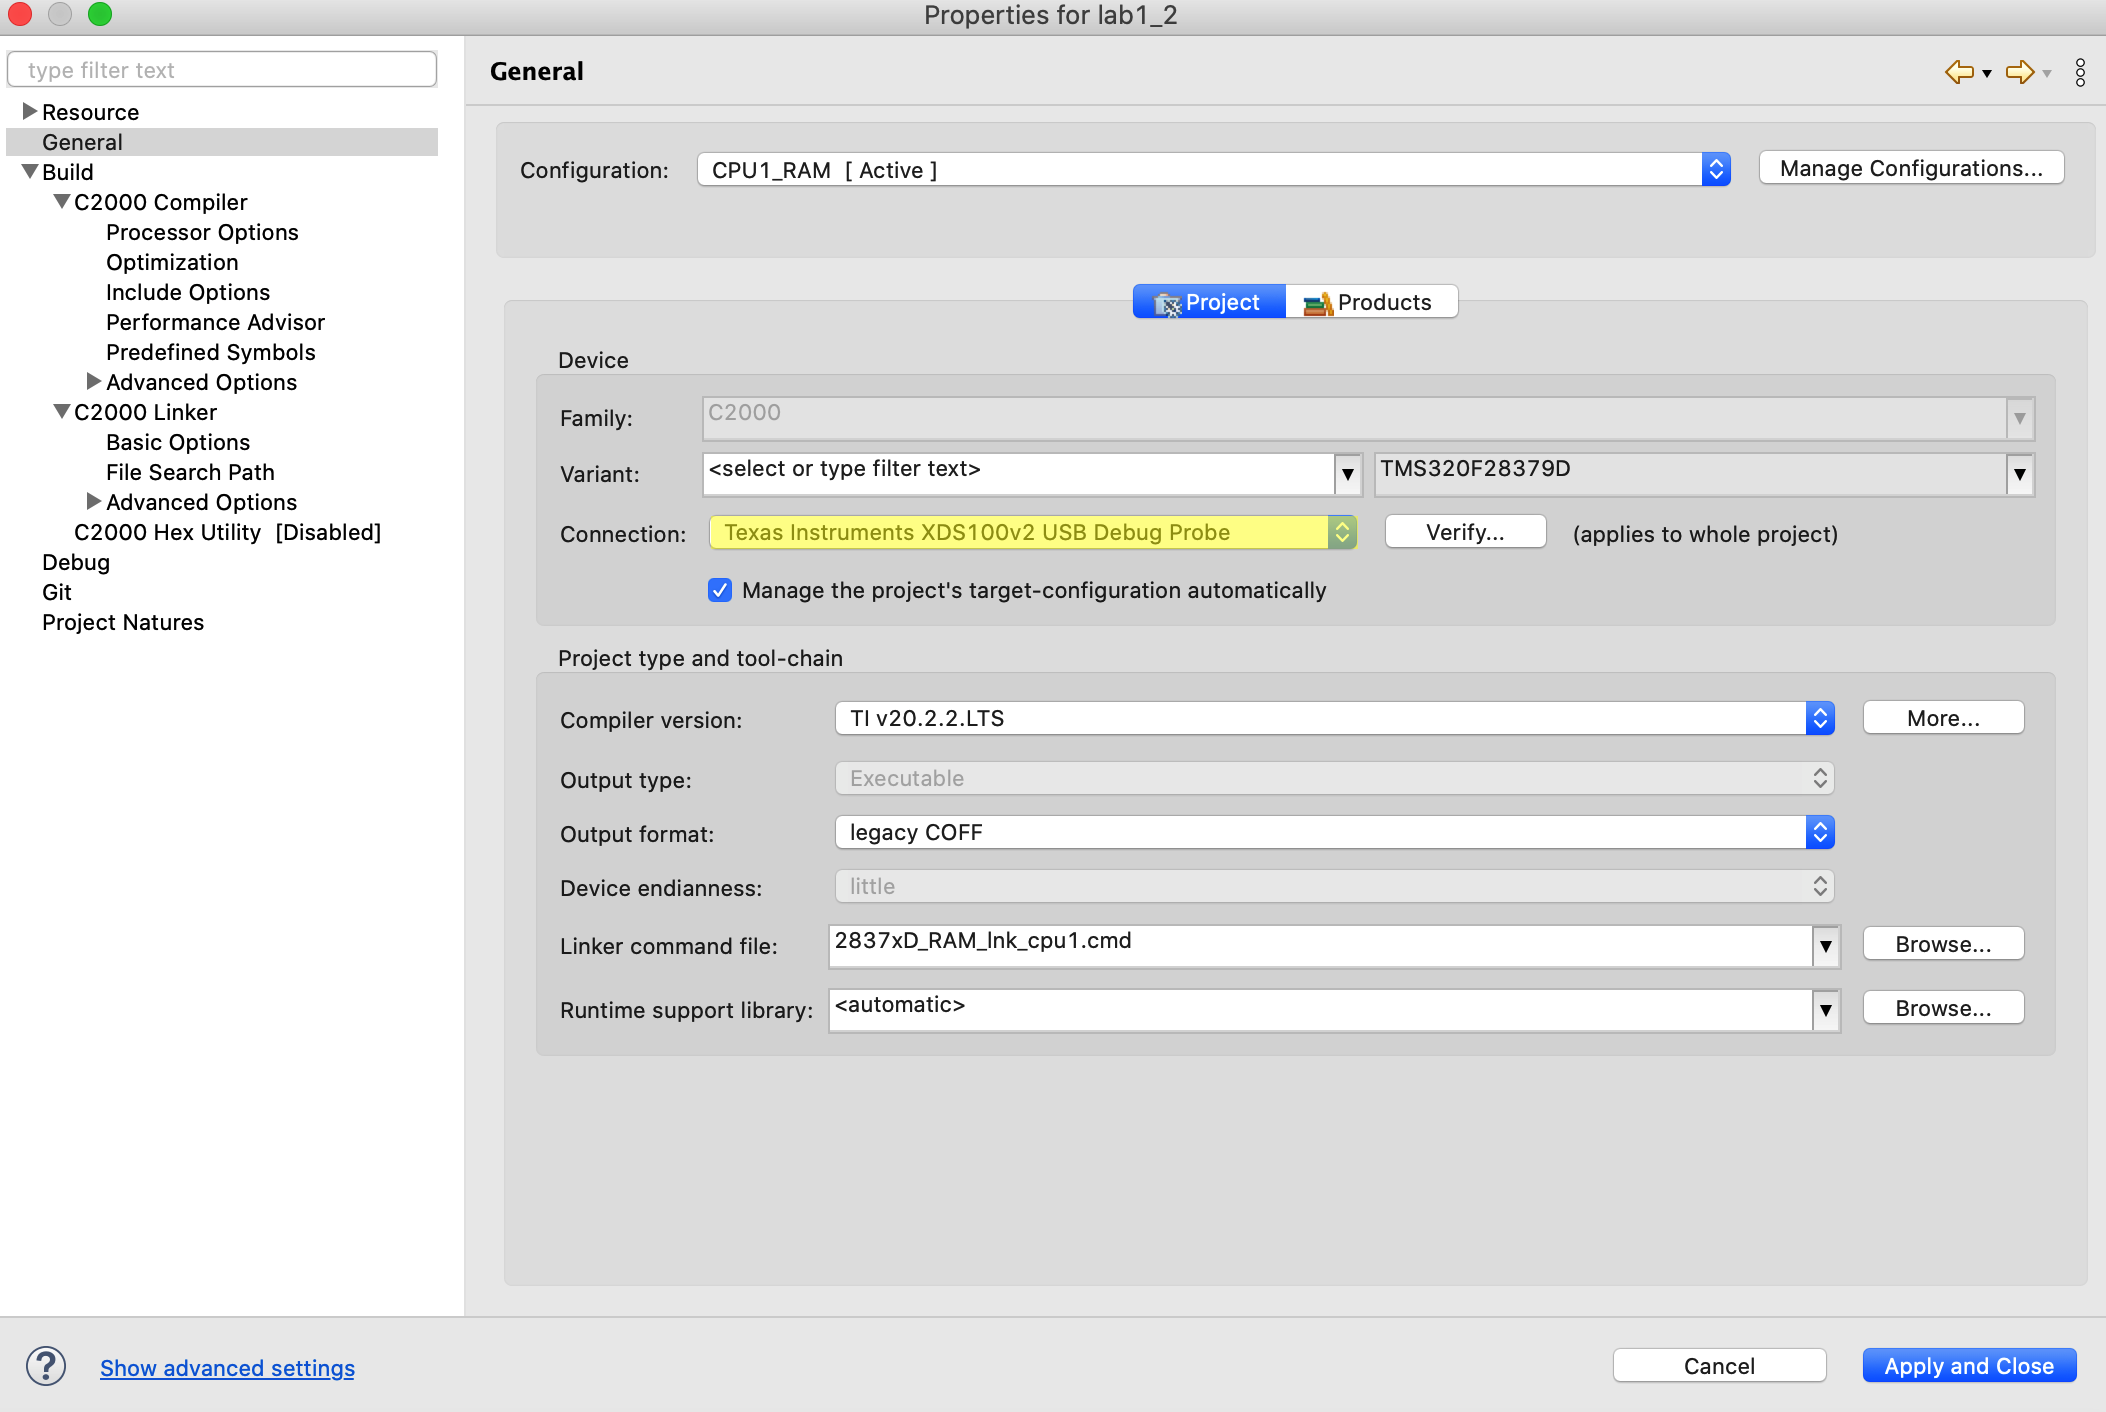
\includegraphics[width = 0.45\textwidth]{ccs_errors_2.png}
\end{figure}

\pagebreak

\section{Serial Terminal}

The \textit{Terminal} application which is a default installation on all Macs can be used as a replacement for the Windows-only \textit{Tera Term} application to interface with a serial port on a Mac. Below are steps to connect to the serial port on a Mac through \textit{Terminal}.

\begin{enumerate}
  \item Open \textit{Terminal}
  \item Type \textit{ls /dev/cu.*} and press \textit{Enter} \\ Example: 
  \begin{figure}[H]
    \centering
    \includegraphics[width = 0.6\textwidth]{step2.png} 
  \end{figure}
  \item Plug in the USB cable from the microcontroller (MSP430, C2x, etc.) to the Mac
  \item Repeat step 2. A new port name should come up that was not there after executing the same command in step 2. It is okay if step 2 was performed with the microcontroller already plugged in. The name of the desired serial port should be something along the lines of \textit{/dev/cu.usbserial-xxxxx} \\ Example:
  \begin{figure}[H]
    \centering
    \includegraphics[width = 0.6\textwidth]{step4.png} 
  \end{figure}
  \item To read from this serial port, type \textit{screen $<$name of port$>$ $<$baud rate$>$} and hit \textit{Enter} \\ Example:
  \begin{figure}[H]
    \centering
    \includegraphics[width = 0.8\textwidth]{step5.png} 
  \end{figure}
  If there are messages on the serial port, the \textit{Terminal} window should now be displaying them. \\
  Example:
  \begin{figure}[H]
    \centering
    \includegraphics[width = 0.6\textwidth]{step5_Ex.png} 
  \end{figure}
  \item To close the serial port, press \textit{CTRL-A} then \textit{CTRL-\textbackslash} and lastly \textit{y} \\
  Example:
  \begin{figure}[H]
    \centering
    \includegraphics[width = 0.6\textwidth]{step6.png} 
  \end{figure}
  \begin{figure}[H]
    \centering
    \includegraphics[width = 0.8\textwidth]{step6_Ex.png} 
  \end{figure}
\end{enumerate}

\subsection{Troubleshooting}
If an error pops up after attempting to follow step 5, make sure that the name of the serial port and baud rate were entered correctly. If this was not the issue, it is likely that a \textit{screen} session is already open. This could result from a previous \textit{screen} session not being terminated correctly (step 6). In this case, the error looks something like
  \begin{figure}[H]
    \centering
    \includegraphics[width = 0.55\textwidth]{step5_Error.png} 
  \end{figure}
  Or, alternatively
  \begin{figure}[H]
    \centering
    \includegraphics[width = 0.55\textwidth]{step5_Error2.png} 
  \end{figure}
To fix this, open \textit{Activity Monitor} and sort the entries alphabetically by clicking the \textit{Process Name} header. Find the process \textit{screen}, double click it, and (force) quit the process. Now retry step 5.
Example:
  \begin{figure}[H]
    \centering
    \includegraphics[width = 0.55\textwidth]{step5_Error3.png} 
  \end{figure}


\pagebreak

\section{Github}

\subsection{Setup}

Navigate to the UIUC Github website at \url{https://github-dev.cs.illinois.edu/} and log in using your university credentials. Once you are given permissions, access the ME461 repository under \url{https://github-dev.cs.illinois.edu/ME461Fall20/Labrepo} and click fork in the top right.

\begin{figure}[H]
    \centering
  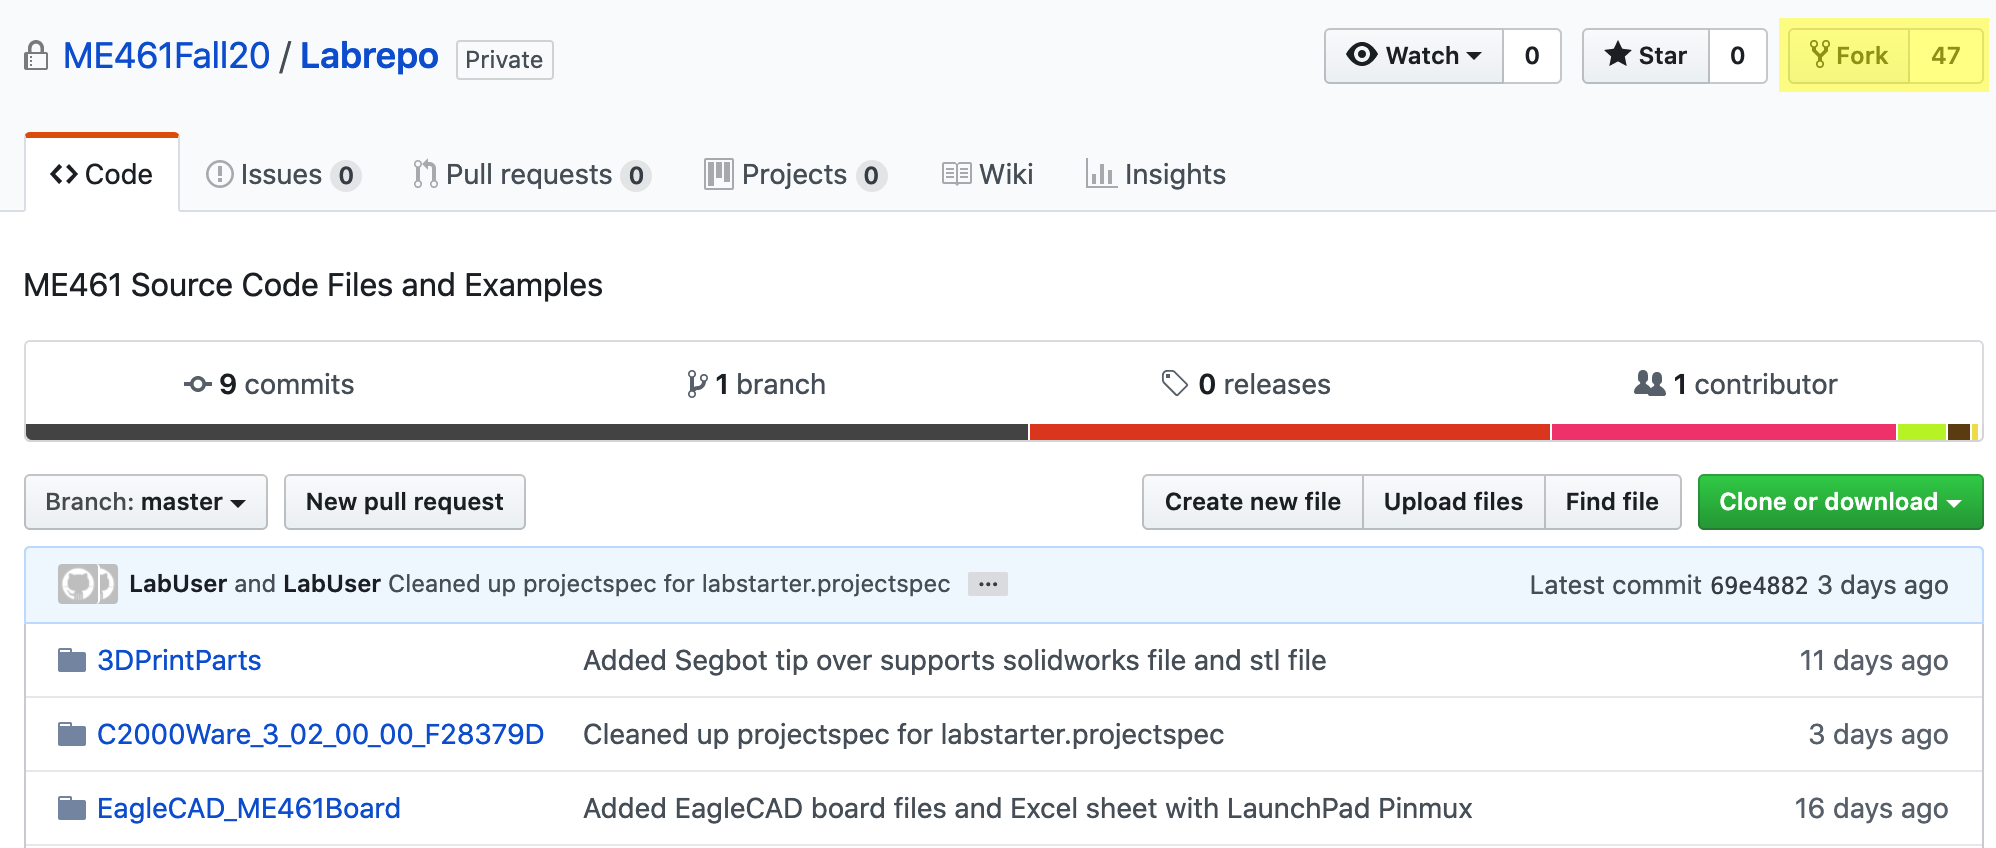
\includegraphics[width = 0.65\textwidth]{github_1.png} 
\end{figure}

This creates a copy of the repository under your credentials. Under settings, rename this to your netID.

\begin{figure}[H]
    \centering
    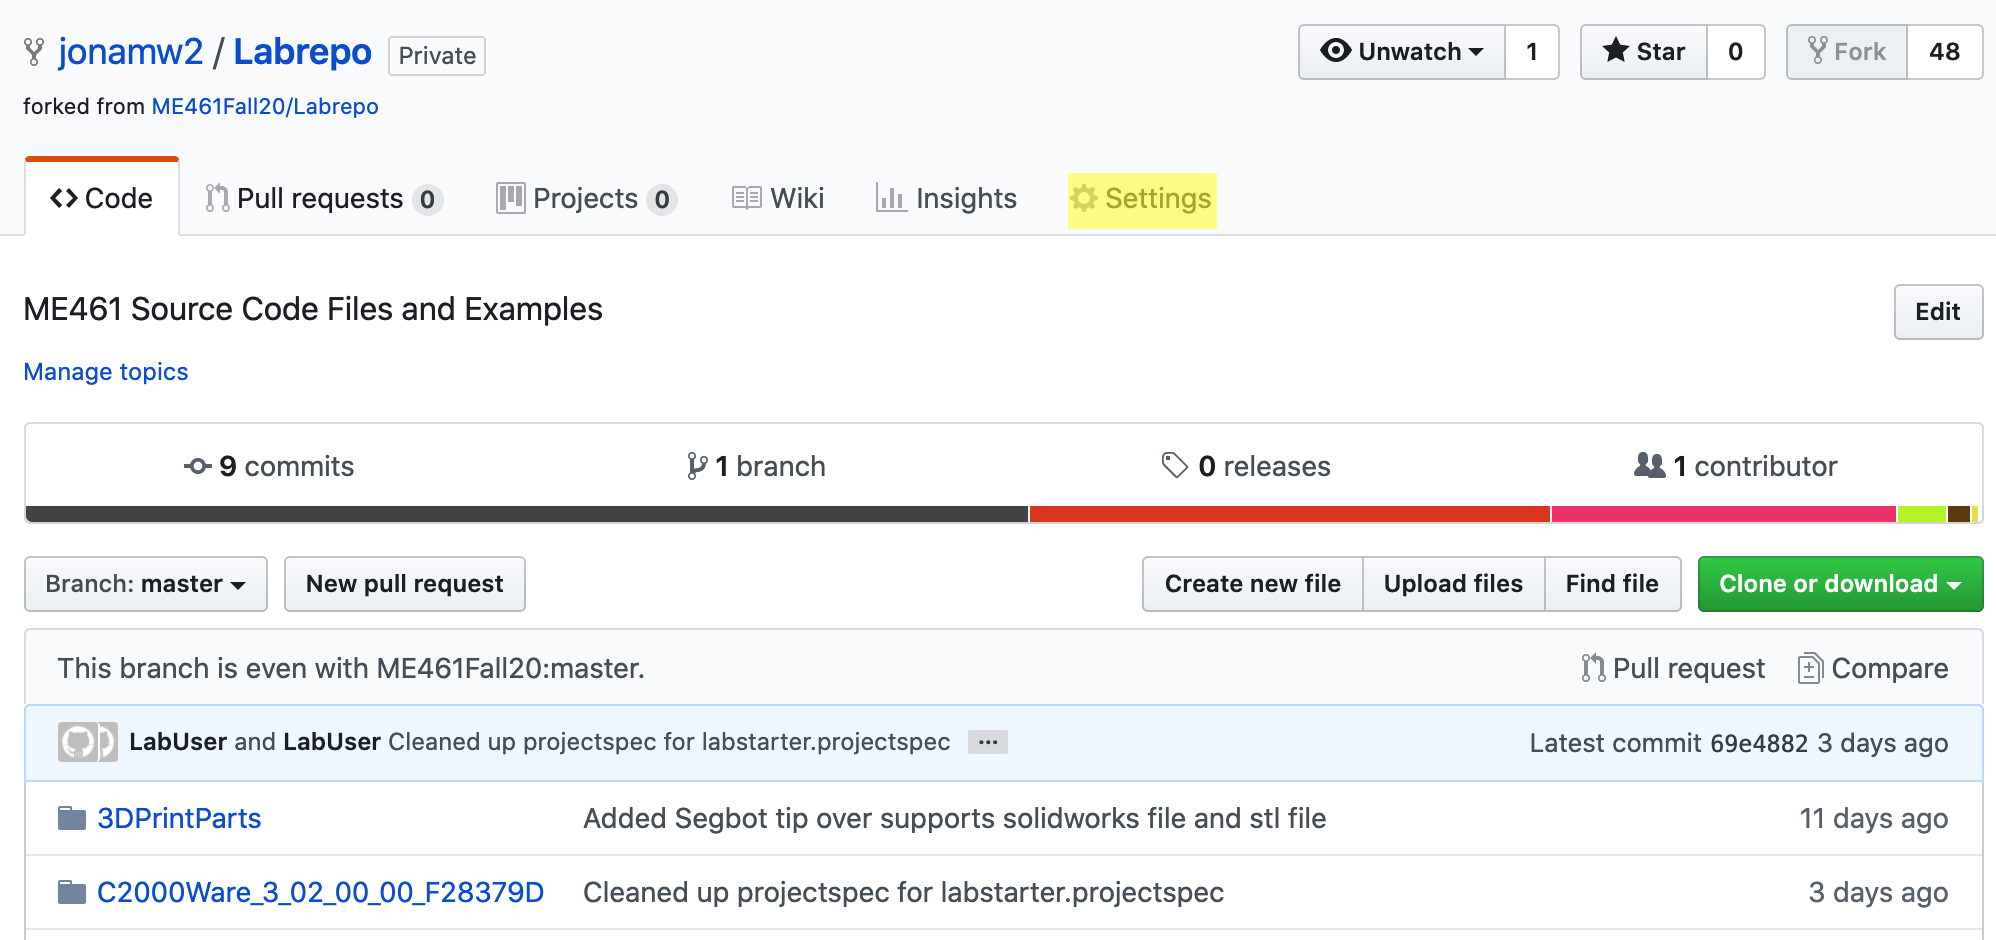
\includegraphics[width = 0.3\textwidth]{github_2.png} 
    \qquad
    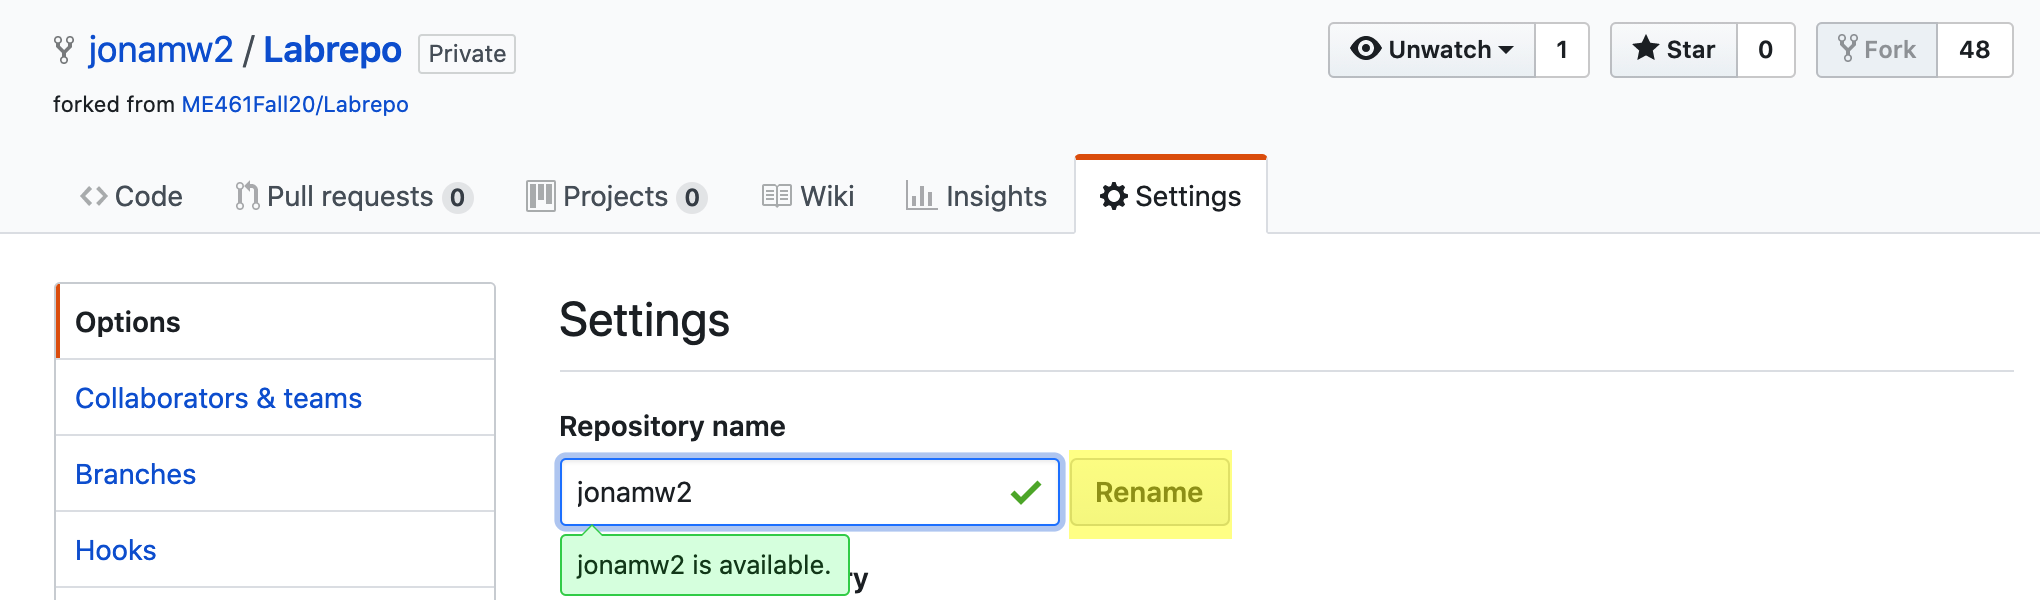
\includegraphics[width = 0.45\textwidth]{github_3.png} 
\end{figure}

Next, under clone or download, copy the URL.

\begin{figure}[H]
    \centering
  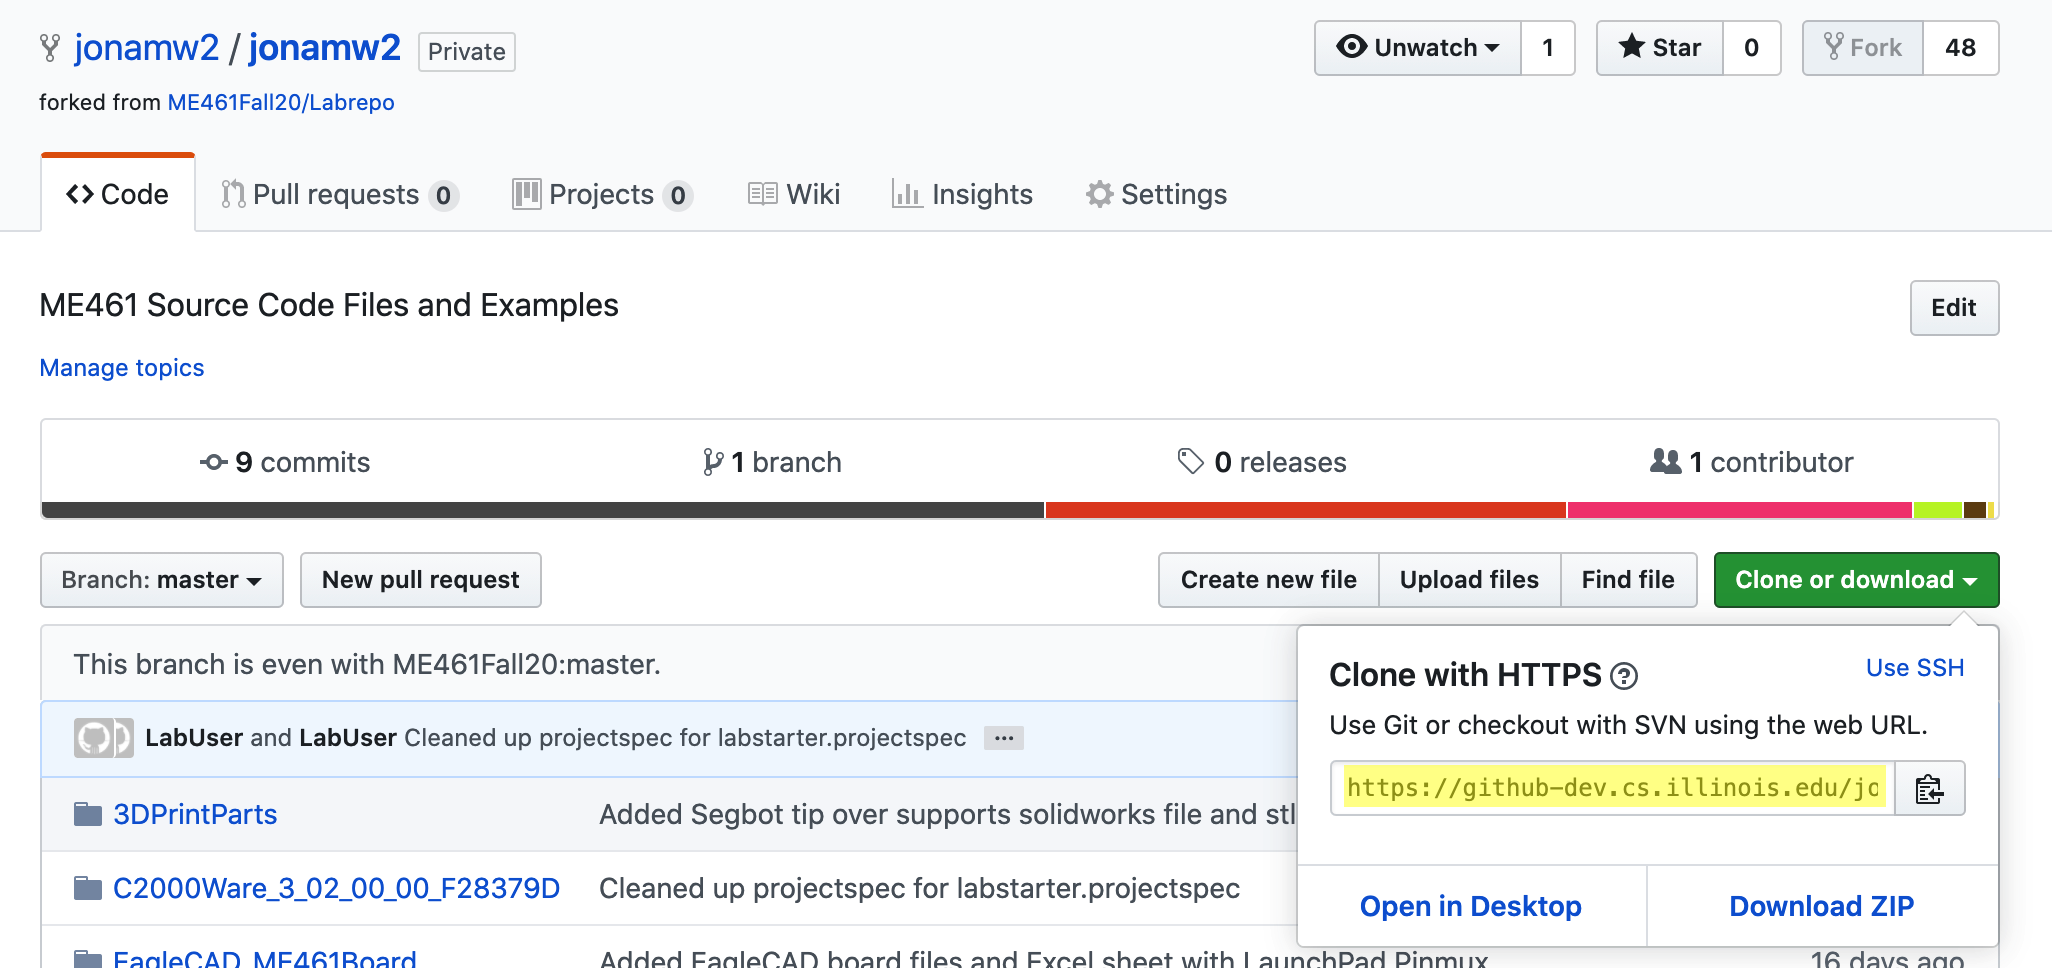
\includegraphics[width = 0.65\textwidth]{github_4.png} 
\end{figure}

Open a terminal window, navigate to where you want the local copy of the repository to be. Then enter \verb|git clone ***| where \verb|***| is replaced by the URL copied in the previous step.

\subsection{Regular Use}

When changes have been made that you want updated, first enter \verb|git add -A|. This both tracks new files and commits them. These commands can be done separately using \verb|git add .| to track and \verb|git commit -a| to commit. It will take you to a vim editor where you need to enter the message in the top line. An alternative is to enter the commit message in the command line:

\begin{center}
    \verb|git commit -a -m "commit message goes here"|
\end{center}

Use \verb|git pull origin master| to sync the master repository and \verb|git push origin master| to push your changes to the remote repository.

\newpage
\subsection{Syncing Personal with Lab Repository}
Step 1 should be run only one time in the history of your local repository. Steps 2-4 should be run every time you want to make sure your local (personal) repository has all the updates from the remote (lab) repository.
\begin{enumerate}
  %%%
  %%% Start of item %%%
  %%%
  \item Run the following line of code to define the branch tracked by your local repository:
  \begin{center}
      \verb|git remote add upstream <original-repo-url>|
  \end{center}
  Example: 
  \begin{figure}[H]
    \centering
    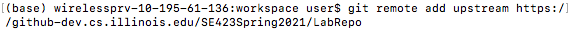
\includegraphics[width = 0.7\textwidth]{Git_Step1a.png} 
  \end{figure}
  This only has to be run once in history of your local repository. However, running it more times should do no harm, only a simple warning will show up stating that the remote upstream already exists. \\ Example: 
  \begin{figure}[H]
    \centering
    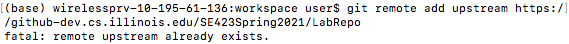
\includegraphics[width = 0.7\textwidth]{Git_Step1b.png} 
  \end{figure}
  To double check whether the remote upstream exists, run the following line of code:
    \begin{center}
      \verb|git remote -v|
  \end{center}
  Two lines beginning with the text \textit{upstream} should show up. \\ Example: 
  \begin{figure}[H]
    \centering
    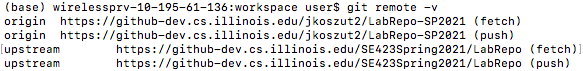
\includegraphics[width = 0.7\textwidth]{Git_Step1c.png} 
  \end{figure}
  %%%
  %%% End of item %%%
  %%%
  %%%
  %%% Start of item %%%
  %%%
  \item To sync your personal repository with the lab repository, first run:
  \begin{center}
      \verb|git fetch upstream|
  \end{center}
  Example: 
  \begin{figure}[H]
    \centering
    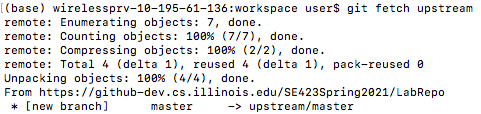
\includegraphics[width = 0.7\textwidth]{Git_Step2a.png} 
  \end{figure}
  Running \textit{git log --oneline} should still show the commit message from your last personal commit.
  \\ Example:
  \begin{figure}[H]
    \centering
    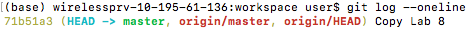
\includegraphics[width = 0.7\textwidth]{Git_Step2b.png} 
  \end{figure}
  Running \textit{git status} should still show that, ``Your branch is up to date with `origin master'."
  \\ Example:
  \begin{figure}[H]
    \centering
    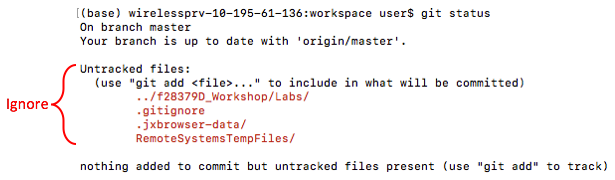
\includegraphics[width = 0.7\textwidth]{Git_Step2c_Annotated.png} 
  \end{figure}
  %%%
  %%% End of item %%%
  %%%
  %%%
  %%% Start of item %%%
  %%%
  \item Next, run:
  \begin{center}
      \verb|git pull upstream master|
  \end{center}
  Example: 
  \begin{figure}[H]
    \centering
    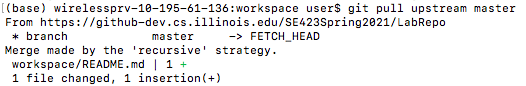
\includegraphics[width = 0.7\textwidth]{Git_Step3a.png} 
  \end{figure}
  Running \textit{git log --oneline} should now show the commit message corresponding to the last commit from the read-only lab repository.
  \\ Example:
  \begin{figure}[H]
    \centering
    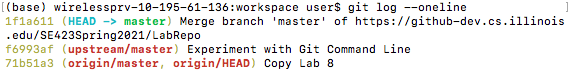
\includegraphics[width = 0.7\textwidth]{Git_Step3b.png} 
  \end{figure}
  Similarly, running \textit{git status} should now show that, ``Your branch is ahead of `origin master'" by at least two commits.
  \\ Example:
  \begin{figure}[H]
    \centering
    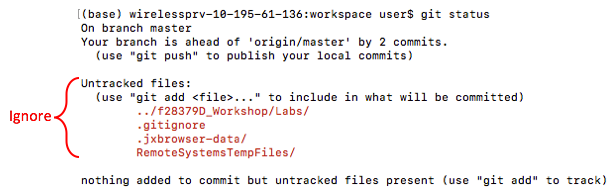
\includegraphics[width = 0.7\textwidth]{Git_Step3c_Annotated.png} 
  \end{figure}
  %%%
  %%% End of item %%%
  %%%
  %%%
  %%% Start of item %%%
  %%%
  \item Lastly, to push the updates from the lab repository to your personal repository, run
  \begin{center}
      \verb|git push origin HEAD|
  \end{center}
  Example: 
  \begin{figure}[H]
    \centering
    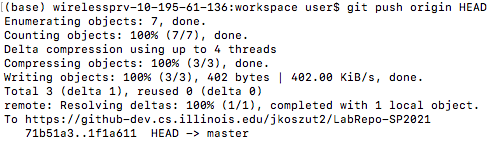
\includegraphics[width = 0.7\textwidth]{Git_Step4a.png} 
  \end{figure}
    Running \textit{git log --oneline} should now show that \textit{origin/master} and \textit{origin/HEAD} line up with the same commit as \textit{HEAD -$>$ master}.
  \\ Example:
  \begin{figure}[H]
    \centering
    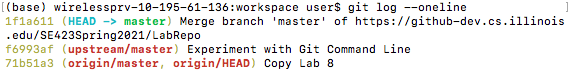
\includegraphics[width = 0.7\textwidth]{Git_Step3b.png} 
  \end{figure}
    Running \textit{git status} should now go back to showing that, ``Your branch is up to date with `origin master'."
  \\ Example:
  \begin{figure}[H]
    \centering
    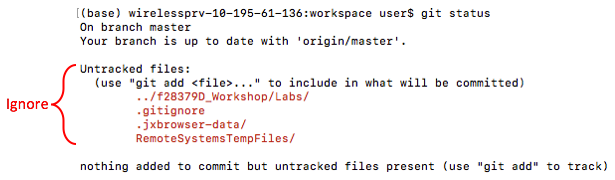
\includegraphics[width = 0.7\textwidth]{Git_Step2c_Annotated.png} 
  \end{figure}
  %%%
  %%% End of item %%%
  To recap, once step 1 has been completed once in your personal repository's history, each time you desire to update your local repository with updates from the lab repository, you only need to run the following three lines of code (steps 2-4):
  \begin{center}
      \verb|git fetch upstream| \\
      \verb|git pull upstream master| \\
      \verb|git push origin HEAD|
  \end{center}
\end{enumerate}


\pagebreak

\section{C Programming}

To set a register use:

\begin{lstlisting}[style=CStyle]
        GpioDataRegs.GPASET.bit.GPIO29 = 1;
\end{lstlisting}

To clear a register, you can't put the set to 0. Instead, use:

\begin{lstlisting}[style=CStyle]
        GpioDataRegs.GPACLEAR.bit.GPIO29 = 1;
\end{lstlisting}

When setting the integer select, set it to the last used SOC, not the channel the last SOC was set to.

\begin{lstlisting}[style=CStyle]
    AdcaRegs.ADCINTSEL1N2.bit.INT1SEL = 0x1; // set to last SOC that is converted and it will set INT1 flag ADCA1
\end{lstlisting}

To setup an interrupt ensure that the corresponding Pievectable register is set to the function name, the correct IER is enabled and the correct PIE is enabled. Be sure before writing to protected registers the command EALLOW is given and then EDIS to disable write ability.

\begin{lstlisting}[style=CStyle]
    PieVectTable.SPIB_RX_INT = &SPIB_isr;
    IER |= M_INT6;  //SPIB
    // Enable SWI in the PIE: Group 6 interrupt 3
    PieCtrlRegs.PIEIER6.bit.INTx3 = 1;
\end{lstlisting}

When writing to the TX Buffers, the register address automatically iterates, so if they are sequentual, after the first, the write address is zero:

\begin{lstlisting}[style=CStyle]
    GpioDataRegs.GPCCLEAR.bit.GPIO66 = 1;
    SpibRegs.SPIFFRX.bit.RXFFIL = 8;
    SpibRegs.SPITXBUF = ((0x8000) | (0x3A00));
    SpibRegs.SPITXBUF = ((0x0000) | (0x0000)); // To address 00x3B write 0x00; To address 00x3C write 0x00
    SpibRegs.SPITXBUF = ((0x0000) | (0x0000)); // To address 00x3D write 0x00; To address 00x3E write 0x00
    SpibRegs.SPITXBUF = ((0x0000) | (0x0000)); // To address 00x3F write 0x00; To address 00x40 write 0x00
    SpibRegs.SPITXBUF = ((0x0000) | (0x0000)); // To address 00x41 write 0x00; To address 00x42 write 0x00
    SpibRegs.SPITXBUF = ((0x0000) | (0x0000)); // To address 00x43 write 0x00; To address 00x44 write 0x00
    SpibRegs.SPITXBUF = ((0x0000) | (0x0000)); // To address 00x45 write 0x00; To address 00x46 write 0x00
    SpibRegs.SPITXBUF = ((0x0000) | (0x0000)); // To address 00x47 write 0x00; To address 00x48 write 0x00
\end{lstlisting}

\end{document}